%============================================================================
% tento soubor pouzijte jako zaklad
% (c) 2008 Michal Bidlo
% E-mail: bidlom AT fit vutbr cz
%============================================================================
% kodovaní: UTF-8 (zmena prikazem iconv, recode nebo cstocs)
%----------------------------------------------------------------------------
% zpracování: make, make pdf, make desky, make clean
%============================================================================
% Šablonu upravil: Ing. Jaroslav Dytrych, idytrych@fit.vutbr.cz
%============================================================================
\documentclass[]{fitthesis} % bez zadání - pro začátek práce, aby nebyl problém s překladem
%\documentclass[zadani]{fitthesis} % odevzdani do wisu - odkazy jsou barevné
%\documentclass[zadani,print]{fitthesis} % pro tisk - odkazy jsou černé
%\documentclass[english,print]{fitthesis} % pro tisk - odkazy jsou černé
% * Je-li prace psana v anglickem jazyce, je zapotrebi u tridy pouzit 
%   parametr english nasledovne:
%      \documentclass[english]{fitthesis}

\usepackage[czech]{babel}
\usepackage[utf8]{inputenc} %kodovani
\usepackage[T1]{fontenc}
\usepackage{cmap}
\usepackage{url}
\DeclareUrlCommand\url{\def\UrlLeft{<}\def\UrlRight{>} \urlstyle{tt}}

%zde muzeme vlozit vlastni balicky
\usepackage{listings}
\usepackage{caption}
\usepackage[toc,page,header]{appendix}
\RequirePackage{titletoc}
\ifczech
  \usepackage{ae}
\fi

\DeclareCaptionFormat{myformat}{#1#2#3}
\captionsetup[lstlisting]{format=myformat}
\captionsetup[lstlisting]{position=bottom,format=myformat}

\lstdefinestyle{JSON}{
    language=Python, 
    showspaces=false,
    showstringspaces=false,
    showtabs=false,
    belowcaptionskip=15pt
}
\renewcommand\lstlistingname{Výpis}
\usepackage{tablefootnote}



%---rm---------------
\renewcommand{\rmdefault}{lmr}%zavede Latin Modern Roman jako rm
%---sf---------------
\renewcommand{\sfdefault}{qhv}%zavede TeX Gyre Heros jako sf
%---tt------------
\renewcommand{\ttdefault}{lmtt}% zavede Latin Modern tt jako tt

% vypne funkci nové šablony, která automaticky nahrazuje uvozovky,
% aby nebyly prováděny nevhodné náhrady v popisech API apod.
\csdoublequotesoff

% =======================================================================
% balíček "hyperref" vytváří klikací odkazy v pdf, pokud tedy použijeme pdflatex
% problém je, že balíček hyperref musí být uveden jako poslední, takže nemůže
% být v šabloně
\ifWis
\ifx\pdfoutput\undefined % nejedeme pod pdflatexem
\else
  \usepackage{color}
  \usepackage[unicode,colorlinks,hyperindex,plainpages=false,pdftex]{hyperref}
  \definecolor{links}{rgb}{0.4,0.5,0}
  \definecolor{anchors}{rgb}{1,0,0}
  \def\AnchorColor{anchors}
  \def\LinkColor{links}
  \def\pdfBorderAttrs{/Border [0 0 0] }  % bez okrajů kolem odkazů
  \pdfcompresslevel=9
\fi
\else % pro tisk budou odkazy, na které se dá klikat, černé
\ifx\pdfoutput\undefined % nejedeme pod pdflatexem
\else
  \usepackage{color}
  \usepackage[unicode,colorlinks,hyperindex,plainpages=false,pdftex,urlcolor=black,linkcolor=black,citecolor=black]{hyperref}
  \definecolor{links}{rgb}{0,0,0}
  \definecolor{anchors}{rgb}{0,0,0}
  \def\AnchorColor{anchors}
  \def\LinkColor{links}
  \def\pdfBorderAttrs{/Border [0 0 0] } % bez okrajů kolem odkazů
  \pdfcompresslevel=9
\fi
\fi

%Informace o praci/projektu
%---------------------------------------------------------------------------
\projectinfo{
  %Prace
  project=BP,            %typ prace BP/SP/DP/DR
  year=2016,             %rok
  date=\today,           %datum odevzdani
  %Nazev prace
  title.cs={Vizualizace síťových bezpečnostních událostí},  %nazev prace v cestine
  title.en={Visualization of Network Security Events}, %nazev prace v anglictine
  %Autor
  author={Petr Stehlík},   %jmeno prijmeni autora
  %author.title.p=Bc., %titul pred jmenem (nepovinne)
  %author.title.a=PhD, %titul za jmenem (nepovinne)
  %Ustav
  department=UPSY, % doplnte prislusnou zkratku: UPSY/UIFS/UITS/UPGM
  %Skolitel
  supervisor=Pavel Krobot, %jmeno prijmeni skolitele
  supervisor.title.p=Ing.,   %titul pred jmenem (nepovinne)
  %supervisor.title.a=,    %titul za jmenem (nepovinne)
  %Klicova slova, abstrakty, prohlaseni a podekovani je mozne definovat 
  %bud pomoci nasledujicich parametru nebo pomoci vyhrazenych maker (viz dale)
  %===========================================================================
  %Klicova slova
  %keywords.cs={Klíčová slova v českém jazyce.}, %klicova slova v ceskem jazyce
  %keywords.en={Klíčová slova v anglickém jazyce.}, %klicova slova v anglickem jazyce
  %Abstract
  %abstract.cs={Výtah (abstrakt) práce v českém jazyce.}, % abstrakt v ceskem jazyce
  %abstract.en={Výtah (abstrakt) práce v anglickém jazyce.}, % abstrakt v anglickem jazyce
  %Prohlaseni
  %declaration={Prohlašuji, že jsem tuto bakalářskou práci vypracoval samostatně pod vedením pana ...},
  %Podekovani (nepovinne)
  %acknowledgment={Zde je možné uvést poděkování vedoucímu práce a těm, kteří poskytli odbornou pomoc.} % nepovinne
}

%Abstrakt (cesky, anglicky)
\abstract[cs]{Tato práce se zabývá vizualizací síťových bezpečnostních dat pomocí moderních webových technologií. Byly studovány různé technologie pro tvorbu moderní webové aplikace podporující vizualizaci velkého množství bezpečnostních událostí. Aplikace byla navržena pro systém NEMEA, který touto prací získal grafické uživatelské rozhraní umožňující vizuální analýzu velkého množství bezpečnostních událostí s možností analýzy shora dolů, tzv. drill-down. Aplikace pracuje s daty uloženými v IDEA formátu, který je využíván dalšími službami z oblasti síťové bezpečnosti a aplikace je tím pádem přenositelná i na ně. Další vývoj aplikace ale bude směřovat k hlubší integraci s NEMEA systémem a jeho službami.}
    
    \abstract[en]{This thesis focuses on visualization of network security events via modern web technologies. Multiple technologies for creating modern web application supporting visualising large volume of security events were studied. The application was designed for NEMEA system which thanks to this thesis acquired graphical user interface allowing big data visual analysis with drill-down capabilities. The application operates on data stored in IDEA format which is used among other network security services and the application is therefore transferrable to them. Further development of the application heads toward deeper integration with NEMEA system and its services.}

%Klicova slova (cesky, anglicky)
\keywords[cs]{JavaScript, Python, MongoDB, vizualizace, NEMEA, IDEA, síťová bezpečnost, SPA}
\keywords[en]{JavaScript, Python, MongoDB, visualization, NEMEA, IDEA, network security, SPA}

%Prohlaseni
\declaration{Prohlašuji, že jsem tuto bakalářskou práci vypracoval samostatně pod vedením pana Ing. Pavla Krobota. Uvedl jsem všechny literární prameny a publikace, ze kterých jsem čerpal.}

%Podekovani (nepovinne)
\acknowledgment{Rád bych poděkoval Ing. Tomáši Čejkovi a Ing. Václavu Bartoši za odbornou pomoc, Ing. Pavlovi Krobotovi za věcné připomínky a vedení během psaní této práce a své rodině a přátelům za podporu.}

\begin{document}
  % Vysazeni titulnich stran
  % ----------------------------------------------
  \maketitle
  % Obsah
  % ----------------------------------------------
  \tableofcontents
  
  % Seznam obrazku a tabulek (pokud prace obsahuje velke mnozstvi obrazku, tak se to hodi)
\ifczech
  \renewcommand\listfigurename{Seznam obrázků}
\fi
  % \listoffigures
\ifczech
  \renewcommand\listtablename{Seznam tabulek}
\fi
  % \listoftables 

  % Text prace
  % ----------------------------------------------
  %=========================================================================
% (c) Petr Stehlík, 2016

%\usepackage{xcolor}
\newcommand\note[1]{{\Large \textcolor{red}{#1}}}

\chapter{Úvod}
Počítačové sítě, zejména Internet, v~dnešním světě zaujímají jednu z~nejvýznamnějších rolí. Počínaje výzkumem a vědeckými experimenty, konče běžným životem většiny lidí. Jen za posledních deset let se počet uživatelů Internetu více než ztrojnásobil. Počítačové sítě propujují celý svět a jsou neustále rozšiřovány, vylepšovány a modernizovány.

Avšak se zvyšujícím počtem uživatelů roste i počet útoků na počítačové sítě. Útočníci se snaží získat citlivé informace či finančně poškodit oběť. Síťový útok je podle~\cite{rfc:attack} definován jako záměrný akt, kde se entita snaží překonat bezpečnostní služby a porušit bezpečnost systému. 

Proto vznikají systémy na detekci síťových útoků, aby správcí sítí dokázali včas a efektivně reagovat na vzniklou situaci. Jeden z~těchto systémů vznikl ve sdružení CESNET s~názvem NEMEA (Network Measurements Analysis). Tento systém mj. slouží pro analýzu síťového provozu a detekci neobvyklých událostí na síti. Podezřelé toky jako agregované události, které pak může systém zaznamenávat do databáze. Takováto událost je uložena ve formátu IDEA. Tento formát je specifikován sdružením CESNET a slouží jako prostředek pro sdílení jednotlivých bezpečnostních událostí mezi různými systémy a bezpečnostními tými.

Na větší síti (stovky až tisíce připojených zařízení) je takovýchto událostí vytvořeno až několik desítek tisíc denně. S~tím nastává problém jak dané události jednoduše a rychle analyzovat a rozpoznat důležité události, na které se zaměřit a na které nebrát zřetel. Pro manuální analýzu velkého množství dat je vhodná vizualizace dle správně zvolených metrik, které vyplývají z~dostupných dat.

Cílem této bakalářské práce je vytvořit aplikaci pro vizuální analýzu bezpečnostních událostí na síti primárně monitorované systémem NEMEA. Nicméně díky formátu dat IDEA, se kterým bude aplikace pracovat, bude možná přenositelnost na další systémy. Důležitým aspektem vytvořené aplikace je důraz na použití moderních nástrojů podporující tvorbu dynamických webových aplikací. Společně s~tím je kladen důraz na uživatelskou přívětivost a jednoduchost prostředí, ve kterém bude probíhat vizuální analýza událostí.

Celou aplikaci navíc bude možno přizpůsobit potřebám daného správce sítě. V~aplikaci bude zavedena technika {\it drill-down}, která napomáhá rychlé a přehledné analýze velkého množství dat bez ztráty informací o~analyzované události. Drill-down spočívá v~postupném zvyšování rozlišení dat, která analyzujeme a postupujeme směřem shora dolů.

Aplikace bude pracovat s~formátem dat nazvaný IDEA. Díky tomu lze aplikaci kdykoliv přenést na jiný zdroj databáze než je systém NEMEA, např. v~rámci sdružení CESNET na systém Warden nebo Mentat. Aplikace bude integrována do systému NEMEA pod názvem NEMEA Dashboard a bude s~ním společně distribuována jako front~end celého systému.

\chapter{Monitorování sítě}

V~rozlehlejších sítích, jako je např. páteřní či firemní síť, je téměř nutností monitorovat a analyzovat provoz na síti, abychom byli informování o~jejím aktuálním stavu, vytížení a zejména negativních vlivech na monitorovanou síť. Samozřejmě i sítě menšího rozsahu by měly být monitorované. Pokud se v~malé firmě podaří útočníkovi infiltrovat síť, výsledky útoku mohou být pro firmu likvidační.

V současné době se provoz analyzuje po tocích, což jsou jednotlivé pakety agregované podle společných metrik a tento záznam je dále zpracováván. To šetří výpočetní výkon a nároky na datový prostor.

Systém pro odhalení průniku (anglicky \uv{Intrusion Detection System}, zkráceně IDS)~\cite{idsips} je takový systém, který analyzuje a identifikuje ze zachyceného provozu podezřelé události. Tyto události může IDS dále klasifikovat. 

\section{IDEA}
\label{sec:idea}

Pro potřebu sdílení informací o~síťových událostech mezi různými skupinami a zařízeními (např. honeypoty, analyzéry systémových zpráv, analyzéry provozu na síti a netflow sondy) existuje několik formátů záznamu pro takovéto události. Nicméně žádný z~nich není natolik univerzální, aby byl vždy a všude použitelný a pokud se k~takovému formátu blíží, tak není natolik detailní, aby pokryl všechny důležité informace.

IDEA\footnote{\url{https://idea.cesnet.cz}}, neboli Intrusion Detection Extensible Alert, je formát záznamu síťové události specifikovaný sdružením CESNET. IDEA si klade za cíl specifikovat takový formát záznamu, který je univerzální, přenositelný, ale zároveň dost konkrétní a snadno pochopitelný bez potřeby rozsáhlé dokumentace k~jednotlivým polím.

Vzorový záznam generovaný systémem NEMEA je vyobrazený ve výpisu \ref{code:idea}. Jak je vidět, formát je specifikovaný jako JSON dokument, aby byl přehledný, čitelný v~běžné podobě (narozdíl od binárních formátů), lehce přenositelný a efektivní (např. oproti XML~\cite{xmlvsjson}).

%\vspace{5mm}
\begin{figure}[ht]
\lstset{basicstyle=\small,style=JSON}
\begin{lstlisting}
{
    "Format" :      "IDEA0",
    "ID" :          "73e0b136-aeb8-4aae-bb80-9bfb4f258847",
    "Category" :    ["Availibility.DDoS"],
    "Description" : "DNS amplification",
    "EventTime" :   "2016-04-07T22:19:25Z",
    "CreateTime" :  "2016-04-07T22:34:52Z",
    "CeaseTime" :   "2016-04-07T22:34:38Z",
    "DetectTime" :  "2016-04-07T22:34:38Z"
    "PacketCount" : 393,
    "Source" : [{
        "IP4" : ["192.1.0.201"],
        "Proto" : ["udp","dns"],
        "OutPacketCount" : 393,
        "InPacketCount" : 767
    }],
    "Target" : [{
        "Proto" : ["udp","dns"],
        "IP4" : ["10.0.0.135"],
        "InPacketCount" : 393
    }],
    "Node" : [{
        "SW" : ["NEMEA","amplification_detection"],
        "Name" : "cz.cesnet.nemea.amplification_detection"
    }],
    "Type" : ["Flow","Statistical"],
}
\end{lstlisting}
\captionof{lstlisting}{Vzorový IDEA záznam ze systému NEMEA. Některé části byly vynechány nebo zkráceny a IP adresy anonymizovány.}
\label{code:idea}
\end{figure}

\newpage

\section{NEMEA}

Network Measurements Analysis (zkráceně NEMEA), je systém, který umožňuje vytvořit komplexní nástroj pro automatizovanou analýzu toků získaných ze síťového monitoringu v~reálném čase. Systém NEMEA je zejména monitorovacím nástrojem, ale slouží také jako IDS.

Systém se skládá z~oddělených stavebních bloků nazývané moduly. Tyto jednotlivé moduly jsou následně propojeny pomocí rozhraní TRAP. Moduly jsou nezávislé pracovní jednotky, které obecně přijímají proud dat na svých vstupech, zpracují či zanalyzují daná data a následně je odešlou ze svých výstupních rozhraní jako proud dat pro další moduly. 

Modul může například tvořit statistiky o~přijatých datech a na základě těchto statistik detekovat určité typy síťového útoku. Detekovaný útok je popsán datovým záznamem, který je odeslán přes výstupní rozhraní dalším modulům, které s~daným záznamem dále pracují, např. jej uloží v~IDEA formátu (viz sekce \ref{sec:idea}) do databáze nebo ze získaných statistik detekují anomálie v~síťovém provozu a dokáží tak jednotlivé pokusy od jednoho útočníka agregovat a zpracovat jej jako jediný útok skládající se z~několika desítek až stovek pokusů o~útok v~delším časovém intervalu a administrátor sítě by je snadno přehlédl nebo ignoroval, pokud by nebyly agregované.

Z~těchto bloků lze postavit i velmi komplexní systém jak je vidět na obrázku \ref{fig:nemea-example-2}, kde jsou data přijímána v~reálném čase z~IPFIX\cite{ipfix} kolektoru. Data jsou předzpracována, analyzována několika algoritmy a následně jsou nahlášeny detekované události. Každá z~těchto úloh je jeden modul, který může být znovu použitý na několika různých místech.

\begin{figure}[h]
    \centering
    \includegraphics[width=1\textwidth]{fig/nemea-example-2-cz.eps}
    \caption{Příklad propojení modulů NEMEA systému, který shromažďuje síťová data, detekuje anomálie a útoky a následně události ukládá a reportuje.} \label{fig:nemea-example-2}
  
\end{figure}


%\subsection*{Hlavní komponenty}

\section{Další monitorovací systémy}

Na trhu jsou v~současné době různá dostupná řešení pro detekci a vizualizaci síťových bezpečnostních událostí, nicméně valná hromada z~nich je komerční a hlavně vázaná na konkrétní hardware od daného výrobce. Klient tudíž většinou nekupuje software, ale hardware s~přiloženým software.

Komerčně dostupný produkt je např. Flowmon ADS~\cite{flowmon:report}\cite{flowmon:ads} od stejnojmenné společnosti. Flowmon je spin-off společností z~projektu Liberouter ze sdružení CESNET. Jejich sondy a kolektory využívají technologie vytvořené ve sdružení CESNET jak z~hlediska hardware, tak software. Dalším komerčním řešením je Cisco Secure IDS~\cite{cisco:ids}, dříve známý jako Cisco NetRanger.

Open source projekty jako NEMEA jsou dostupné mnoho let, ale pouze několik z~nich dosáhlo znatelnějšího rozšíření v~komunitě síťových správců. Nejvýznamnějšími jsou systémy Snort~\cite{snort}, VERMONT~\cite{vermont} a framework Bro~\cite{bro}. 

\subsection*{Snort}
Tento open-source projekt, od roku 2013 vlastněn firmou Cisco~\cite{snort:cisco}, je možno konfigurovat ve 3 hlavních režimech~\cite{snort:modes}: sniffer, paket logger a jako IDS. V~režimu IDS Snort pracuje principiálně velmi podobně jako systém NEMEA. Zachytává síťový provoz, ukládá si důležité informace o~něm a analyzuje jej. Ve výsledku ukládá záznamy o~síťových událostech. Nicméně Snort není modulárním systémem a tudíž není tak flexibilní a není stavěný na vysokorychlostní rozsáhlé sítě jako systém NEMEA.

\subsection*{VERMONT}

VERMONT (Versatile Monitoring Toolkit) je modulární monitorovací systém obsahující IPFIX kolektor, exportér, analyzátor a další moduly a grafické prostředí pro vizuální analýzu dat. VERMONT byl vyvinut v~rámci projektu HISTORY~\cite{vermont:history} a evropským projektem DIADEM firewall~\cite{vermont:diadem}. Svou architekturou je nejbližší systému NEMEA, protože je částečně modulární. Systém NEMEA je oproti tomu modulární od samotného jádra systému, což dovoluje vyšší flexibilitu při vývoji a menší závislost na použitých technologií.

\subsection*{Bro}
Dalším, v~komunitě rozšířeným řešením, je framework Bro. Tento framework primárně určený pro síťovou analýzu není podobný systému NEMEA, ani předchozím systémům, protože je to spíše nástroj pro vytváření (N)IDS než-li ucelený systém. Bro se velmi blíží skriptovacímu jazyku (např. Perl) nebo unixovým nástrojům jako tcpdump nebo nfdump. Bro lze rozdělit na dvě vrstvy. První vrstvou je \uv{Bro Event engine}, který analyzuje síťový provoz a generuje neutrální síťové události v~podobě \uv{byla vytvořena nějaká událost}. 

Tyto neurčité události jsou následně analyzovány druhou vrstvou -- \uv{Bro Policy skripty}. V~této vrstvě je implementovaný zmiňovaný skriptovací jazyk. V~současné době existuje mnoho naprogramovaných skriptů, které jsou připraveny k~okamžitému použití, včetně pokročilé analýzy síťového provozu.

V~ranných fázích vývoje se systém NEMEA velmi blížil frameworku Bro, s~vývojem času se ale NEMEA stala uceleným systémem připraveným k~okamžitému nasazení na měřící body.

\section{Shrnutí}

V~této kapitole jsme prezentovali systém NEMEA a jeho architekturu. Popsali jsme jeho nejdůležitější části, zejména jak vypadá modul a jeho komunikační protokol. Dále jsme popsali formát záznamu síťové bezpečnostní události IDEA, který je opěrným bodem pro ukládání dat v~systému NEMEA v~rámci analýzy událostí koncovým uživatelem. V~poslední sekci jsme porovnali systém NEMEA s~dalšími veřejně dostupnými monitorovacími systémy.

%%%%%%%%%%%%%%%%%%%%%%%%%%%%
% Kapitola 3
% Technologie
%%%%%%%%%%%%%%%%%%%%%%%%%%%%

\chapter{Technologie}

Vizualizace síťových bezpečnostních událostí může být vytvořena několika postupy. Pokud máme IDS, který je dostupný pouze z~jednoho stroje, nejčastěji zvolíme tvorbu desktopové aplikace, protože máme jistotu provozního prostředí jako je např. operační systém, dostupné balíčky a jejich verze. 

V~případě vzdálené správy IDS (častější případ) jsme nejčastěji odkázání na vzdálený přístup pomocí příkazové řádky. Tento přístup je bohužel velmi limitovaný a nelze jej využít pro vizualiaci. V~současné době je pro vzdálenou správu nejvhodnější vytvořit webovou aplikaci, která je dostupná z~Internetu a použitelná na většině dnes používaných zařízeních\footnote{Jedná se zejména o~stolní počítače, notebooky, tablety a chytré mobilní telefony.}.

Pro tvorbu moderních webové aplikace je na Internetu dostupná celá řada knihoven, frameworků a systémů. Nicméně první otázkou zůstává co taková moderní webová aplikace je?

Ustáleným pojmem pro moderní webovou aplikaci je z~anglického single page application~\cite{spa} (zkratka SPA). Specifikem SPA je její vysoká interaktivita s~uživatelem, vysoká dostupnost služby, kterou poskytuje a rozdělení na dva logické celky. Uživatelskou a serverovou část, často chybně nazývané frontend a backend aplikace. Více o~architektuře aplikace v~kapitole \ref{architektura}.

Většinu z~těchto kvalit získává SPA díky způsobu jakým je doručována uživateli. SPA je při prvním načtení stránky v~prohlížeči celá uložena v~rámci vyrovnávací paměti prohlížeče a během celé doby použivání SPA není nutné stránku znova načítat. SPA můžeme chápat jako univerzálního klienta pro obsluhu dané aplikace. 

SPA je nejčastěji tvořena pomocí jazyka JavaScript. Ten umožňuje dynamickou změnu stránky bez nutnosti ji znova načítat a tím pádem uživatel nepřichází o~dočasná data na stránce. Tento přístup navíc redukuje počet dotazů na server a snižuje tak jeho zátěž.

S~přesunem logiky na uživatelskou část SPA jsou ale spojeny nemalé problémy. Zejména pak různorodá interpretace kódu. To se v~posledních letech téměř eliminovalo díky moderním prohlížečům a jejich jádrům jako je např. WebKit pro Google Chrome nebo Gecko pro Firefox.

\section{Uživatelská část}

K~vytvoření SPA a zejména uživatelské části existuje několik významných systémů. V~této části tyto technologie budou představeny a porovnány mezi sebou. Nejdůležitější částí je JavaScriptový framework, se kterým bude interagovat uživatel. Další nedílnou součástí je knihovna pro HTML/CSS definující vzhled aplikace.

\subsection{JavaScriptové frameworky}

V rámci této práce bylo vybráno 5 JavaScript frameworků, které napomáhají k~tvorbě SPA. Kritéria užšího výběru frameworků byla zejména následující:

\begin{itemize}  
\item open-source projekt s~licencí pro volné použití,
\item jednoduché použití,
\item nenáročný na výpočetní výkon hostitelského stroje,
\item široká podpora mezi prohlížeči,
\item projekt má historii a je vyvíjen některou ze známých společností (udržitelnost vývoje).
\end{itemize}

\subsubsection*{React~\cite{react}}
Knihovna React je vyvíjena pod hlavičkou společnosti Facebook. Původním cílem návrhářů Reactu bylo vyřešit problémy během vývoje komplexních uživatelských rozhraní s~rychle měnícími se daty. Dalším cílem bylo vytvořit platformu, kterou lze distribuovat v~takovém měřítku jako je Facebook.

React je knihovna pro uživatelskou část SPA používající tradiční MVC architekturu~\cite{mvc}. Taková architektura je nejvíce znatelná v~případě použití obousměrného vázání dat (anglicky two-way data binding), více v~sekci \ref{sec:mvc}.

React se zaměřuje zejména na tvorbu uživatelského rozhraní\footnote{Z~pohledu MVC architektury na pohledovou část (angl. view).} a kvůli tomu se ostatním částem architektury nevěnuje tak detailně, jak by většinu času vývojář potřeboval. Velmi častým řešením je použít React na pohledovou část a na model a kontrolér použít jiný framework, např. AngularJS.

React pracuje s~moderními přístupy k~vývoji SPA a boří tak mnoho zažitých technik jak takovou SPA vyvíjet. Místo běžné manipulace s~DOM elementy si React, případně vývojář, definuje vlastní DOM\footnote{Angl. Document Object Model je konvence pro objektovou reprezentaci a interakci s objekty v HTML dokumentu.} elementy.

Těmto elementům dynamicky mění jejich obsah, manipuluje s nimi a to bez větších výkonových ztrát. Toho docílil zejména použitím tzv. shadow DOM~\cite{shadowdom}, který je ale novinkou na poli prohlížečů a je podporován pouze jádrem WebKit\footnote{Využívá jej např. prohlížeč Google Chrome nebo Safari.}. 

%Pokud není shadow DOM dostupný, používá React standardní DOM, se kterým je sice vykreslování pomalejší, ale stále velmi rychlé. 

\begin{figure}[ht]
\lstset{basicstyle=\small,style=JSON}
\begin{lstlisting}
var HelloMessage = React.createClass({
    render: function() {
        return <div>Hello {this.props.name}</div>;
    }
});

ReactDOM.render(<HelloMessage name="World" />, mountNode);
\end{lstlisting}
\captionof{lstlisting}{\uv{Hello World} příklad v~jazyku JSX, který do stránky vykreslí text \uv{Hello World}.}
\label{code:react}
\end{figure}

Pro názornou ukázku, jak framework React funguje, je ve výpise \ref{code:react} vytvořen jednoduchý \uv{Hello World} element v~JSX~\cite{jsx} syntaxi. Tento kód demonstruje pouze minimální možnosti frameworku, ale vypovídá o~jednoduchosti použití Reactu.

\subsubsection*{Ember.js}

Ember.js je primárně zaměřen na tvorbu SPA. Toho dosahuje obsáhlou funkcionalitou bez nutnosti instalace dalších doplňků a osvědčil se i vysokou stabilitou během celé doby vývoje. Ember je také vždy jedním z~prvních frameworků, který implementuje novinky obsažené v~nových jádrech webových prohlížečů jako jsou např. JavaScript Promises~\cite{jspromises}, Web Components~\cite{webcomponents} nebo ES6 syntaxe.

Ember se skládá celkem z~pěti klíčových konceptů:

\begin{itemize}  
    \item {\bf Cesty} (angl. routes) -- každý stav aplikace je reprezentován unikátní cestou a této cestě náleží i odpovídající objekt, který manipuluje s~danou cestou.
    \item {\bf Modely} (angl. models) -- každá cesta má svůj korespondující model, který obsahuje data asociována s~danou cestou a stavem aplikace. Model slouží zejména k~manipulaci s~daty.
    \item {\bf Šablony} (angl. templates) -- šablony jsou tvořeny v~HTML s~použitím šablonovacího jazyka HTMLBars~\cite{htmlbars}. Do této šablony jsou při vykreslování stránky dynamicky navázány na proměnné v JavaScript kódu Ember.js. 
    \item {\bf Komponenty} (angl. components) -- komponenta je vlastní HTML značka definovaná programátorem aplikace. Její chování je implementováno pomocí JavaScriptu a její vzhled pomocí HTMLBars šablon. Komponenta se chová jako běžný DOM element.
    \item {\bf Služby} (angl. services) -- servis je singleton\footnote{Během doby běhu aplikace lze vytvořit pouze jednu instanci třídy.} objekt, který v~sobě udržuje dlouhodobá data během používání aplikace klientem.
\end{itemize}

\subsubsection*{AngularJS}

AngularJS je jedním z~nejdéle existujících frameworků pro tvorbu SPA. Je vyvíjen společností Google a poskytuje ucelené prostředí k~vývoji komplexních SPA. AngularJS poskytuje dvě metodiky návrhu architektury aplikace. MVC a MVVM (model-view-viewmodel)~\cite{mvvm}.

MVVM je rozdílný zejména ve způsobu nakládání s~daty v~aplikaci. Viewmodel pouze reflektuje změny modelu v~pohledu a naopak. Ten lze chápat také jako interpret dat získaných z~modelu, které jsou požadovány v~pohledu.

Vzhledem k~rozsáhlosti knihovny se nevyhneme tvorbě aplikace, která prolíná oba typy architektury. AngularJS je ale založen na základech MVC architektury.

AngularJS staví na třech základních pravidlech:

\begin{itemize}
    \item odddělit manipulaci DOM a aplikační logiku,
    \item diferenciovat klientskou a serverovou stranu aplikace,
    \item poskytnout strukturu pro vývoj SPA.
\end{itemize}

Manipulace s~DOM je zajišťována v~pohledové části architektury. Aplikační logika je oddělena, což umožňuje simultánní tvorbu na obou částech aplikace. To dovoluje strukturovat kód do uzavřených logických celků, které mohou být znovu použity v~dalších částech aplikace.

Rozdělením klientské a serverové strany aplikace získává AngularJS celkovou kontrolu nad klientskou stranou a dokáže tak abstrahovat jednotlivé vrstvy aplikace. To integruje MVC architekturu do klientské části.

Toto rozdělení dovoluje AngularJS implementovat takové možnosti jako je např. vkládání závislostí (pozdní instanciace daných závislostí) nebo pohledově závislé kontroléry (daný kód je spouštěn pouze při daném pohledu).

To vše spěje ke snížení zátěže serveru, na kterém je SPA uložena. Většina, ne-li všechna, aplikační logiky totiž probíhá na klientské straně a server pro svou práci vůbec nepotřebuje. Ten je potřeba až v~momentě kdy chceme získat nebo uložit data pro dlouhodobé užití.

\subsubsection*{Backbone.js}

Framework Backbone.js se mírně odlišuje od předešlých a to svou architekturou, která není MVC, ale MVP (model-view-presenter). Prezentér je v~tomto případě prostředníkem, který plní logickou funkci a spojuje pohled s~modelem. Veškeré akce, které se provedou v~pohledu (např. kliknutí na tlačítko) jsou delegovány prezentéru. Ten je navíc oddělen od pohledu a komunikuje s~ním pouze přes definované rozhraní.

Tento přístup je vhodný zejména pro testování a jasné oddělení jednotlivých částí (zvláště modelu od pohledu). Avšak MVP je náročnější na tvorbu kvůli tomu, že všechny datové vazby musí vytvořit sám programátor.

Výhodou Backbone.js je jeho velikost (celková velikost distribuce je méně než 8 kB) a nezávislost na dalších knihovnách (vyžaduje pouze jednu další knihovnu\footnote{Underscore.js, pokud chce programátor využít i složité funkce, musí navíc doplnit knihovnu jQuery.}).

Z~předcházejících faktů lze vyvodit, že Backbone.js je vhodný zejména pro SPA menšího rozsahu, které jsou zaměřeny na velmi konkrétní úkol. To může v~pozdějších fázích vývoje SPA znamenat problémy a kompromisy při vývoji další funkcionality aplikace.

\subsubsection*{Shrnutí}

Pro rychlý a stručný přehled byla vypracována tabulka shrnující klíčové vlastnosti každého porovnávaného frameworku.

\begin{table}[ht]
\centering
\caption{Porovnání klíčových vlastností JavaScript frameworků}
\label{tab:js}
\begin{tabular}{|l|l|l|l|l|}
\hline
    Název       & 
    Verze\tablefootnote{Aktuální verze v~době psaní této práce.}     & 
    Aktivní vývoj     & 
    Velikost\tablefootnote{Velikost komprimovaného produkčního kódu.}  & 
    Licence   \\ \hline
    React       & 15.0.1    & 3 roky (2013)     & 142 kB    & BSD       \\
    Ember.js    & 2.5.0     & 4 roky (2011)              & 450 kB    & MIT       \\
    Backbone.js & 1.3.3     & 5 let (2010)              & 7.5 kB    & MIT       \\
    AngularJS   & 1.5.3     & 5 let (2010)              & 152 kB    & MIT       \\
\hline
\end{tabular}
\end{table}

\newpage

\subsection{HTML/CSS frameworky}

Důležitým aspektem SPA je také její vzhled, nebo spíše UX (user-experience)~\cite{ux:iso}. UX je zejména vnímání a reakce osoby, které plyne z~používání nebo předpokládaného užití/chování výrobku, systému nebo služby. Důraz se musí klást zejména na předpokládáné chování systému, tím pádem může uživatel procházet plynule aplikací, aniž by musel odhadovat chování té části aplikace, ve které se právě nachází.

Toho lze dosáhnout zejména uceleností vzhledu a chování jednotlivých komponent SPA. Pro tento účel existují tzv. HTML/CSS knihovny. Na Internetu je jich velké množství a v rámci této práce byl výběr zúžen na tři běžně používané knihovny mající širokou škálu komponent, které lze v~SPA využít a jejich zdrojové kódy jsou volně dostupné.

Zdrojové kódy jazyka CSS by měly být vytvořeny v~jednom z~CSS preprocesorů~\cite{css:preproc} -- LESS\footnote{\url{http://lesscss.org}} nebo SASS\footnote{\url{http://sass-lang.com}}, aby v~aplikaci byla zaručena konzistence proměnných (např. barvy, velikost, odsazení).

\subsubsection*{Bootstrap}

Bootstrap je velmi populární knihovnou pro tvorbu vzhledu SPA. Obsahuje HTML a CSS komponenty pro ucelenou typografii, formuláře, tlačítka, navigaci a další. Bootstrap také nabízí komponenty, které jsou částečně nebo zcela napsány v~JavaScriptu.

Bootstrap je udržován zejména společností Twitter, kde také vznikl na popud tvorby interních firemních aplikací s~uceleným vzhledem a také UX, aby se ušetřily náklady na údržbu takovýchto aplikací.

Díky Bootstrapu se velmi rychle ujal trend responzivního designu a mobile-first přístupu. Navíc disponuje velkou komunitou vývojářů a časté problémy jsou tak mnohokrát vyřešeny.

\subsubsection*{Foundation}

Foundation je velmi podobný framework jako Bootstrap. Také nabízí HTML a CSS komponenty pro různé části SPA včetně JavaScript komponent, je neméně kvalitní (z hlediska vývojáře) a udržovaný.

Hlavním rozdílem oproti Bootstrapu je jeho upravitelnost. Foundation dává větší prostor pro úpravu jednotlivých komponent. 

Navíc disponuje styly, které jsou automaticky aplikované na dané HTML elementy -- vývojář nepotřebuje přidávat množství tříd ke každému elementu. To však nemusí každému vyhovovat a mohou nastat neobvyklé konflikty aplikovaných stylů během vývoje.

\subsubsection*{Angular Material}

Angular Material není běžnou CSS knihovnou, nýbrž je velmi úzce spjat s~AngularJS a využívá jeho mnoha možností jako jsou např. vlastní HTML elementy (direktivy).

Také obsahuje mnoho HTML a CSS komponent, ale ty jsou vždy velmi úzce spjaty s~AngularJS funkcionalitou jako je např. two-way data binding a již zmíněné direktivy. 

Společnost Google disponuje vizuálním jazykem pro všechny své produkty nazvaný Material Design\footnote{\url{https://www.google.com/design/spec/material-design/introduction.html}}. Ten je založený na tzv. \uv{kartách}, které lze skládat na sebe, řadit, organizovat a upravovat. Jak již název napovídá, je tento vizuální jazyk použit skrz všechny dostupné komponenty.

Z~technického hlediska je Angular Material nejpokročilejší knihovnou. Pro mřížkový systém (angl. grid system) používá flexbox~\cite{flexbox}, který je dostupný pouze v~nejnovější specifikaci CSS 3 a moderních webových prohlížečích. To může působit mírné problémy, pokud je SPA cílena na široké publikum s~různými verzemi prohlížečů.


\section{Serverová část}

V~rámci serverové části je kladen důraz zejména na poměr výkonnost/spotřeba zdrojů, stabilitu a efektivitu programu. Tyto faktory jsou ovlivněny zejména použitým programovacím jazykem, knihovnami a návrhem architektury programu.

Požadavkem pro server v této práci je, aby byl typu Unix/Linux. To nám zaručuje určité faktory a vlastnosti provozního prostředí jako např. dostupné jazyky a jejich knihovny, podpůrné programy a další.

Z aplikace NEMEA Dashboard bude na serveru spuštěno REST API\footnote{Rozhraní pro programování aplikací, angl. application programming interface.}~\cite{rest}(viz kapitola \ref{architektura}). API se připojuje na NoSQL databázový systém MongoDB. Ta je využívána systémem NEMEA pro ukládání detekovaných událostí. MongoDB bylo zvoleno kvůli rychlosti, jednoduchosti použití a pro záznamy ve formátu IDEA bylo potřeba NoSQL databázový systém, který dokáže pracovat s~daty stejně nebo podobně jako se pracuje s~formátem JSON.

\subsection{REST API}
\label{crud}

REST, neboli Representational State Transfer, je architektura rozhraní pro distribuci dat. Tato architektura dovoluje přistupovat ke všem zdrojům jednotným rozhraním, které definuje čtyři základní operace nad každým z~nich:

\begin{description}
    \item {\bf Create} -- vytvoření a uložení nového datového objektu.
    \item {\bf Read} -- čtení datového objektu.
    \item {\bf Update} -- permanentní aktualizace datového objektu.
    \item {\bf Delete} -- odstranění datového objektu z~permanentního datového prostoru.
\end{description}

Toto rozhraní (zkráceně CRUD) zpřístupňuje databázi událostí vytvořenou NEMEA systémem a udržovánou v~MongoDB. Navíc tato data agreguje, předzpracovává či jinak upravuje (funkcionalita REST API je popsána v~sekci \ref{restapi})

Pro vytvoření API s~REST architekturou rozhraní existují knihovny, které vývoj ulehčují a zrychlují. Ve většině případů ale platí, že takovéto knihovny jsou náročné na zdroje a jsou tím pádem pomalejší. Pro NEMEA Dashboard je potřeba takový jazyk, který je úzce integrovaný se systémem a dokáže využívat systémové nástroje\footnote{Využití systémových nástrojů není součástí této práce, ale byla jednou z~podmínek návrhu REST API pro NEMEA Dashboard.}.

Do výběru jsem zahrnul interpretované i kompilované jazyky, aby byl demonstrován rozdíl ve výkonnosti, jednoduchosti použití, množství potřebných závislostí a dalších faktorů. Jmenovitě byly zahrnuty jazyky Python, C++ a JavaScript. Pro každý vybraný jazyk existuje několik knihoven pro podporu tvorby REST API, proto pro zpřehlednění byly vybrány knihovny, se kterými mám předešlé zkušenosti.

Jeden z~nejpoužívanějších jazyků pro tvorbu webových stránek -- PHP nebyl zahrnut z~důvodu vysoké režie interpretu při běhu aplikace a mnoha závislostí (zejména Apache webový server), které jsou potřeba pro tvorbu webové stránky v~PHP. Navíc jazyk PHP přímo nepodporuje tvorbu REST architektury, vše je řešeno přes Apache server pomocí .htaccess konfigurace.

\subsubsection*{Flask (Python)}

Flask je tzv. mikroframework, čímž vývojáře nenutí využívat konkrétní knihovny nebo nástroje, nedisponuje žádnou abstraktní databázovou vrstvou, verifikací vstupů nebo kteroukoliv jinou komponentou běžně dostupnou ve frameworku podobného typu.

Nicméně Flask podporuje rozšíření, kterými lze rozšířit funkcionalitu přesně dle potřeb programátora. Tím se stává Flask velmi silným nástrojem při vývoji SPA.

Veškeré zde zmíněné skutečnosti dělají z Flask ideální nástroj pro návrh jak rozsáhlého, tak minimálního REST API, které lze libovolně škálovat dle potřeb projektu.

S~ohledem na MongoDB existuje konektor PyMongo vytvořený autory MongoDB. Ten se použitím velmi podobá příkazové řádce přímo v~MongoDB. 

\subsubsection*{NodeJS (JavaScript)}

JavaScript je původně určen do prostředí webových prohlížečů a jejich jader. Společnost Google ale vytvořila V8~\cite{google:v8} JavaScriptové jádro primárně určené pro webový prohlížeč, na kterém je postaven i nástroj NodeJS. V8 umožňuje spouštět kód napsaný v~JavaScriptu na straně serveru.

Architektura NodeJS je založena na principu asynchronních událostí, které dovolují vytvářet vysoce škálovatelné síťové aplikace, jako je např. webový server s~vysokou dosupností.

NodeJS není až tak knihovnou nebo nástrojem pro vývoj webových serverů, jako spíše sbírkou modulů, které obsluhují jednotlivé části funkcionality jádra~\cite{nodejs}. Tyto moduly využívají API, které zjednodušuje komunikaci mezi moduly. Tím se velmi podobá NEMEA systému.

\subsubsection*{Mongoose (C/C++)}

Posledním kandidátem je framework napsaný v~jazyku C. Největší výhodou tohoto řešení je jeho rychlost, která je násobně vyšší než u~interpretovaných jazyků\footnote{Z měření (viz \ref{serv:fin}) až 40 krát rychlejší než Python.}. Mongoose je minimalistický framework vytvořený pro vývoj webových serverů více typů.

Jelikož jazyk C není až tak pohodlný a rychlý pro vývoj abstraktních architektur rozhraní jakou je REST, zejména kvůli práci s~textovými řetězci a manipulací s~JSON objekty, rozhodl jsem se napsat obálku frameworku Mongoose do jazyka C++\footnote{Tato obálka byla vytvořena mimo rozsah této práce pro jiný projekt.}. Ten je vhodnější pro práci s~textovými řetezci a existuje efektivní knihovna pro práci s~JSON objetky RapidJSON~\cite{js:rjson}.

Za použití vytvořené obálky, která je navržena specificky pro návrh REST API, lze velmi rychle vytvořit požadovanou funkcionalitu. Obálka totiž doplňuje možnosti Mongoose, který např. nedisponuje dynamickými URL\footnote{z angl. uniform resource locator} nebo zpracováním URL parametrů do vhodné struktury.

Největším problémem je absence oficiálního konektoru pro MongoDB, ten je nezbytnou podmínkou pro toto REST API. Existují různá řešení nebo knihovny. Ty jsou ale buď neudržované nebo náročné na použití.

\section{Vybrané technologie}

V~předcházející kapitole byl uveden užší výběr technologií, které jsou vhodné pro tvorbu SPA jak z~uživatelské, tak serverové části. Každá z~nich je něčím specifická a vyčnívá oproti jiným kandidátům.

\subsection{Uživatelská část}

Prvními aspekty při výběru knihovny pro vývoj SPA v~uživatelské části byla zejména velikost knihovny, množství dostupných modulů, licence, udržovatelnost a v~neposlední řadě dostupné funkce. Pro rychlý přehled byla vytvořena tabulka \ref{tab:js}, která některé z těchto faktorů porovnává.

Licence BSD a MIT jsou velmi podobné z~pohledu vývojáře a jejich možnostmi použití v~rámci vývoje otevřeného projektu jakým je NEMEA.

Z~hlediska velikosti jasně vyčnívá EmberJS, který je násobně menší než ostatní frameworky, avšak z~ostatních faktorů pozbývá funkcionalitu, kterou např. dokáže nabídnout AngularJS.

Všechny frameworky jsou v~současné době aktivně vyvíjeny a pravidelně aktualizovány. Navíc kolem každého frameworku, které jsou všechny open-source, je vytvořena aktivní komunita vývojářů, kteří přispívají do daného frameworku.

Pokud se zaměříme na možnosti frameworku, jasně vybočuje AngularJS, který implementuje kompletní MVC/MVVM architekturu. Tím pádem není nutná jakákoliv další knihovna nebo vlastnoruční implementace některých komponent, které budou při vývoji NEMEA Dashboard potřeba.

Poslední faktor -- možnosti frameworku -- je dle mého nejdůležitějším měřítkem při výběru. Ten totiž vyváží i větší velikost frameworku a jeho náročnost na prohlížeč, ta se navíc s~každou novou verzí většinou snižuje.

Tím pádem je jasným vítězem framework AngularJS, který disponuje širokou funkcionalitou. Je navržený přímo pro vývoj komplexních SPA a má mnoho dostupných rozšíření.

Volba AngularJS značně ovlivnila výběr CSS knihovny, protože Angular Material je přímým rozšířením frameworku AngularJS a do útrob Angular Material je velmi hluboce integrovaný. Navíc používá nejmodernější technologie, které usnadňují vývoj.

\subsection{Serverová část}
\label{serv:fin}

Při výběru technologie pro serverovou část byl kladen důraz zejména na rychlost výsledného REST API a jeho udržitelnost z~vývojářského hlediska (modulárnost, OOP\footnote{Objektově orientované programování.}). Proto jsem vytvořil velmi jednoduché REST API v~každém z~kanditátů a změřil jejich výkonnost.

V~každém z~frameworků jsem vytvořil jednoduché statické API (fixní URL), která vrátilo textový řetězec \uv{Hello World}. Pro měření jsem využil virtuální server s~následujícími parametry:

\begin{itemize}
    \item CPU -- Intel(R) Xeon(R) CPU W3520  @ 2.67GHz (2 jádra),
    \item RAM 1GB DDR3 ECC,
    \item rychlost připojení do Internetu -- 500 Mbps.
\end{itemize}

Server nebyl v~době testů nijak vytížen a běžely na něm pouze základní služby. Pro vytvoření dostatečného množství dotazů na server jsem použil nástroj wrk\footnote{\url{https://github.com/wg/wrk}}. Ten byl spouštěn s~následujícími parametry:

\begin{itemize}
    \item \texttt{-d 20s} -- délka trvání testu,
    \item \texttt{-t 10} -- počet vláken,
    \item \texttt{-c 200} -- počet otevřených připojení,
    \item URL.
\end{itemize}

Testy byly spouštěny celkem třikrát pro každý framework, aby se vyvarovalo chybě měření a každé měření probíhalo nezávisle na předcházejícím. Stejný server se nikdy netestoval dvakrát za sebou. V~tabulce \ref{tab:server} jsou zaznamenány naměřené výsledky.

\begin{table}[ht]
\centering
\caption{Naměřené vlastnosti serverových frameworků pomocí nástroje wrk}
\label{tab:server}
\begin{tabular}{|l|l|l|l|l|}
\hline
    Název       & Celkem požadavků  & Požadavků/s   & Latence   & Vytížení CPU\\ \hline
    Flask       & 3 373             & 167.9         & 25.82 ms  & ~25\%\\
    NodeJS      & 117 579           & 5871.6        & 33.60 ms  & ~130\%\\
    Mongoose    & 136 001           & 6787.5        & 29.80 ms  & ~100\%\\
   \hline
\end{tabular}
\end{table}

C++ obálka frameworku Mongoose a NodeJS jsou několikanásobně rychlejší než framework Flask. V případě C++ obálky je tomu díky použitému jazyku a NodeJS je koncipovaný pro multivláknovou síťovou komunikaci. Ten jediný v základu podporuje vícevláknové zpracování požadavků. 

Ačkoliv se může zdát, že NodeJS je jasnou volbou z~naměřených výsledků, není tomu tak. NodeJS totiž během testu spotřeboval téměř všechny zdroje daného stroje (zejména CPU). Díky tomu je natolik výkonný. Tohoto výkonu lze dosáhnout i u~frameworku Flask, ale ten by musel být doplněn dalšími nástroji pro efektivní vícevláknové zpracování požadavků.

Pokud bychom pracovali v~izolovaném prostředí, je nejvhodnější NodeJS. Pokud ale budeme vycházet z~architektury aplikace, zjistíme, že REST API nesmí být upřednostňováno před databází. V~ní totiž probíhají mnohem náročnější operace, které vytvářejí prodlevu v~odpovědi v~rámci sekund a ne jednotek milisekund jako v~případě serveru. 

Flask je v poměru rychlost/spotřebované zdroje nejvhodnějším kandidátem, navíc díky implementaci v~Pythonu je velmi jednoduchý na použití, s~udržitelným kódem a pohodlnou prací s~JSON objekty. Pokud bychom se zaměřili na rychlost, lze dosáhnout dobrých výsledků zapojením CPython. Navíc Python nedovolí spotřebovat veškeré zdroje stroje, což se stalo při testu Mongoose a zejména pak NodeJS serveru.

\section{Shrnutí}

Vybrané technologie jsou vyváženou kombinací široké funkcionality, rychlosti vývoje a udržitelnosti kódu. To platí jak pro uživatelskou, tak serverou část aplikace.

Pro uživatelskou část jsem vybral JavaScript framework AngularJS společně s~CSS frameworkem Angular Material, ty se navzájemně doplňují funkcionalitou a jsou úzce provázány.

Serverová část bude realizována v~jazyku Python pomocí mikroframeworku Flask. Ten disponuje všemi potřebnými funkcionalitami pro tvorbu REST API a MongoDB disponuje konektorem PyMongo pro jazyk Python, který je snadný na použití a má široký repertoár funkcí a nastavení.

\chapter{Architektura aplikace}
\label{architektura}

Před samotnou implementací aplikace je potřeba navrhnout její architekturu. Ačkoliv se SPA může jevit jako jednoduchá a přímočará struktura, opak bývá většinou pravdou. Bez nutnosti načítání stránky uživatel nevnímá změnu mezi jednotlivými pohledy v~aplikaci. Ta se ale v~pozadí asynchronně dotazuje na server a procházení stránky je tak velmi plynulé.

Celá SPA byla již při výběru technologií rozdělena na dva logické celky. Uživatelskou a serverovou část. Schéma \ref{fig:system} znázorňuje architekturu SPA a kde jsou jaké technologie použité.

\begin{figure}[ht]
    \centering
    \includegraphics[width=0.5\textwidth]{fig/SPA.pdf}
    \caption{Rozvržení SPA na dva logické celky a jaké technologie tyto celky používají.} \label{fig:system}
\end{figure}

Díky použitým technologiím lze části rozdělit aplikačně i fyzicky na dva stroje. Serverová část je spustěna na jednom počítači -- serveru, jenž je určen pouze pro databázi a REST API. Server tedy zajišťuje funkčnost REST API a při iniciální návštěvě klienta také poskytuje kód uživatelské části, který je spuštěn u klienta.

Tím se distribuuje uživatelská část aplikace na samotná zařízení, která aplikaci zobrazují. Následkem je snížení nároků na serverovou část obstarávající pouze datovou a autentikační část SPA (vše uvnitř REST API).

Největší využití bude mít v~aplikaci dashboard (odtud i název aplikace), který bude obsahovat konfigurovatelné položky, aby si uživatel mohl Dashboard připravit přesně pro své potřeby. Dashboard je také vstupním bodem pro drill-down analýzu.

\section{Případy užití}
Před samotným návrhem architektury byly určeny čtyři případy užití, ze kterých vychází návrh pro NEMEA Dashboard. Tyto navržené případy zohledňují širokou škálu úkonů, které při běžném používání IDS mohou nastat.

Jako cílová skupina uživatelů jsou uvažování správci větších sítí. Ti musí být informováni o~stavu spravované sítě. Většinou jsou takovéto sítě stavěny velmi robustně a jsou dostatečně naddimenzovány. Neobvyklé událostí na síti je ale nutné monitorovat a předcházet jim.

\label{sec:aud}

\begin{description}
    \item \textit{Běžný přehled o~síti a analýza provozu z~několika posledních dní} \\
        Správce sítě musí mít přehled o~síti, kterou spravuje. Chce být informován o~celkovém počtu útoků, které detekoval systém NEMEA a ty následně uložil jako události. Správce nechce pročítat emailové reporty nebo ručně procházet jednotlivé události. Proto chce využít NEMEA Dashboard pro zobrazení významných událostí a agregovaného pohledu na ně.
    \item \textit{Detekce útoku většího rozsahu na síť} \\
        Při běžné analýze sítě pomocí NEMEA Dashboard musí být útok okamžitě vidět ve zobrazených datech. Většinou se takovýto útok nahlásí jako velké množství menších útoků. V~tu chvíli je pro správce velmi těžké takový útok odhalit, pokud data nebudou vizualizována a agregována.
    \item \textit{Analýza nezvyklé události} \\
        Uživatele zaujala velmi nezvyklá událost a chce o~ní zjistit více. Postupně se dostává k~detailnějším informacím pomocí drill-down analýzy. Na konci analýzy vidí podrobné detaily o události (jako jsou např. IP adresa zdroje a cíle, typ události, jaký modul ji reportoval, atp) a může tak podniknout další kroky jako např. změnit konfiguraci firewallu, aby blokovalútočníka, informovat oběť emailem, případně podniknout další opatření.
    \item \textit{Kontinuální přehled o~síti} \\
        Uživatel během své běžné pracovní činnosti Dashboard sleduje pasivně, tzn. dashboard se autonomně aktualizuje a uživatel vidí aktuální dění na síti. Velmi jednoduchou a rychlou vizuální analýzou (běžným pohledem) identifikuje událost, která se právě vyskytla na síti s~krátkou časovou prodlevou (v~rámci jednotek minut).
        
\end{description}

Tyto případy užití lze rozdělit do dvou typů dat. Vizualizovaná data pomocí grafů a textové informace o~uložených událostech v~daný časový interval. Z~toho lze vyvodit několik základních typů zobrazovaného obsahu pro dashboard:

\begin{itemize}
    \item graf podílů (koláčový graf) -- ukazuje podíly událostí dle kategorie v~definovaném časovém okně,
    \item graf v~čase (sloupcový graf) -- zobrazuje množství událostí rozdělené v~intervalech v~definovaném časovém okně dle kategorií,
    \item informace o~nejvýznamnějších (tzv. top-N) událostech (text) -- největší události dle statického pole v~databázi v~určitém časovém okně.
    \item informace o~celkovém počtu (text) -- celkový počet detekovaných událostí v~určitém časovém okně,
\end{itemize}

Ze tří prvních uvedených zobrazovaných prvků bude možná drill-down analýza. V~případě grafů bude možnost prokliku na výpis událostí, které jsou filtrované dle odpovídajících atributů (např. kategorie a čas). U~boxu s~nejvýznamnějšími událostmi bude odkaz přímo na detail dané události.

Další částí NEMEA Dashboard bude přehled všech událostí nazvaný jednoduše \uv{Events}. Zde bude možnost vyhledávat a třídit všechny události, které se v~databázi nacházejí. Všechny vyhledané a vyfiltrované události budou přehledně zobrazeny v~tabulce, která bude obsahovat základních informace o~události. U~každé události bude možnost prokliku k~detailním informacím, které jsou o~události uloženy v~databázi.

Poslední částí aplikace budou nastavení. Ty v~rámci této práce budou pouze pro uživatele a jejich správu (přidání, editace a smazání uživatele).

\section{Uživatelská část}
\label{sec:mvc}
Architektura uživatelské části je definována knihovnou AngularJS, která využívá MVC architekturu. Ta spočívá v~rozdělení aplikace na tři logické celky, které návzájem spolu komunikují a předávají si data.

\begin{figure}[ht]
    \centering
    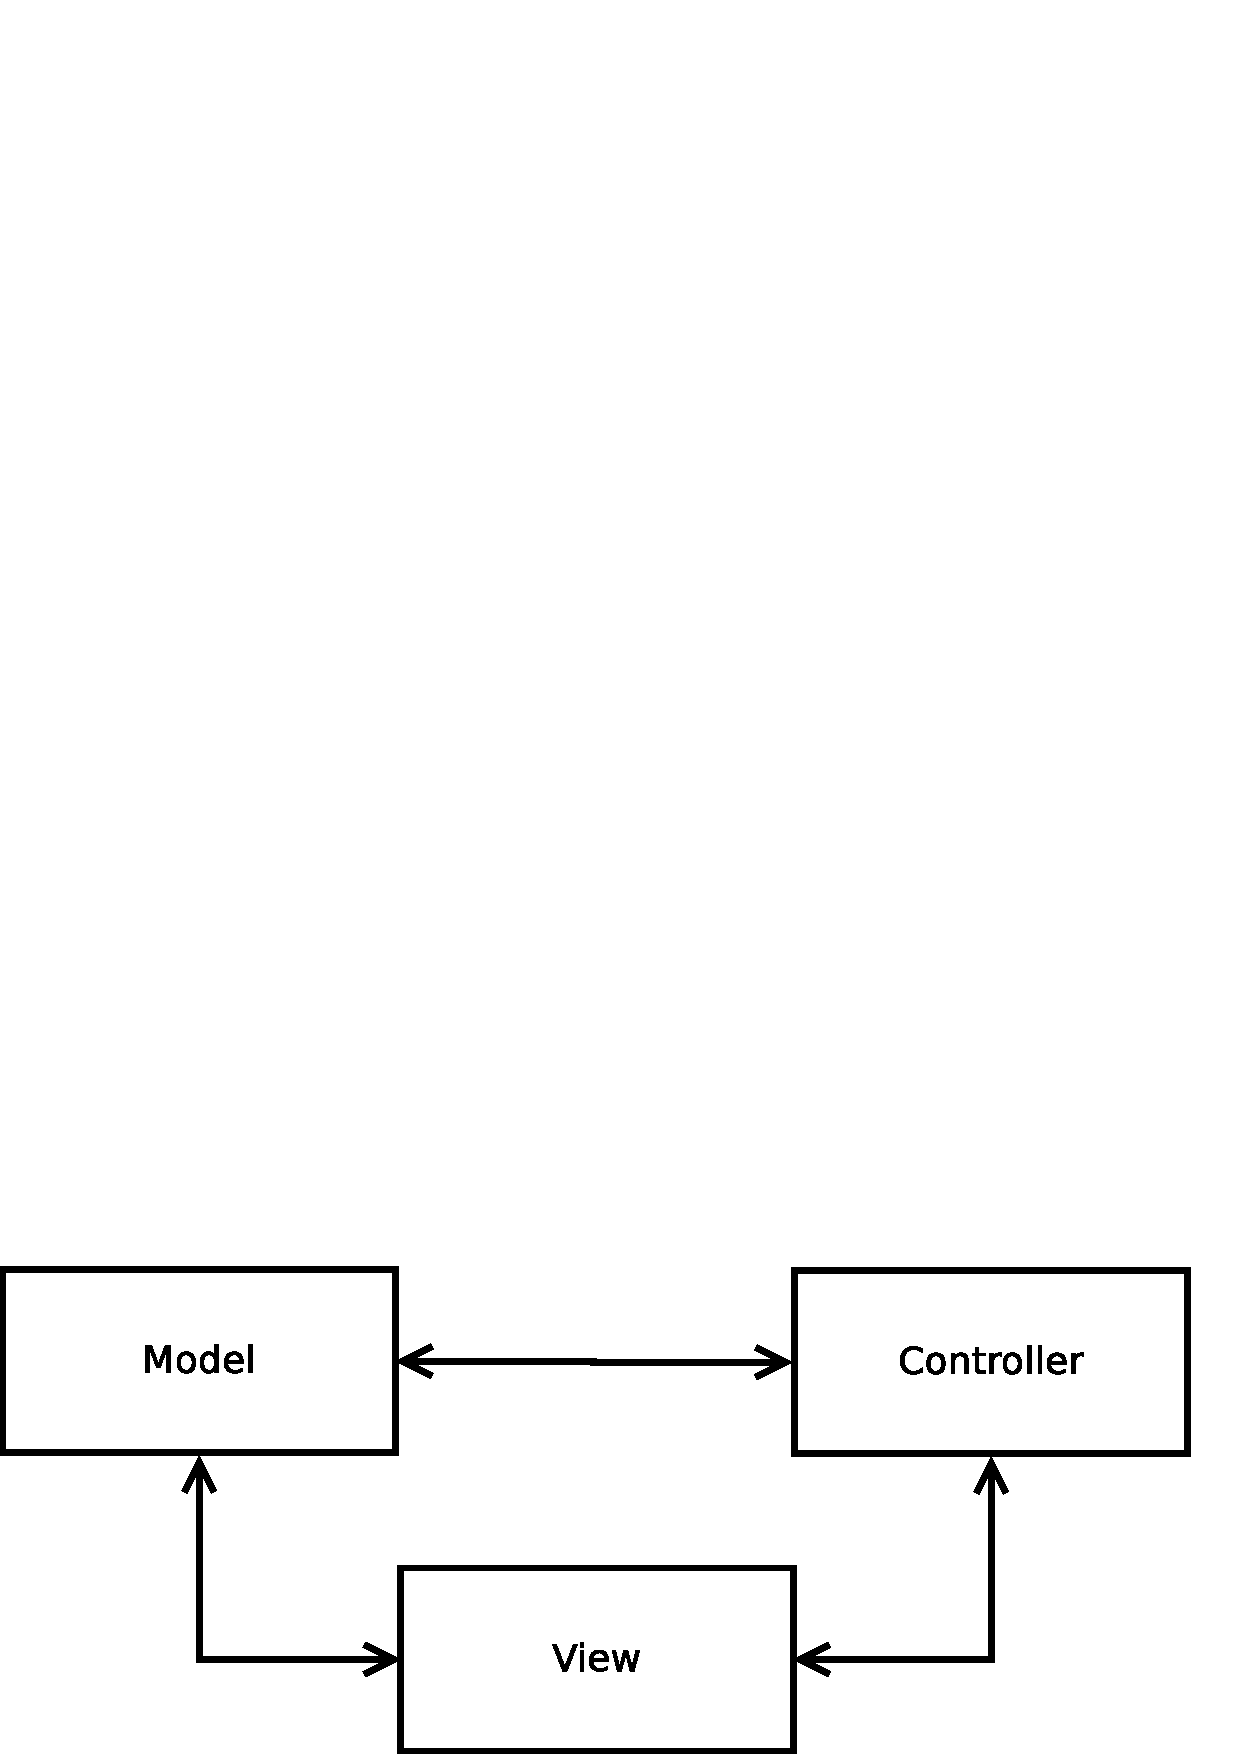
\includegraphics[width=0.5\textwidth]{fig/mvc.pdf}
    \caption{MVC architektura} \label{fig:mvc}
\end{figure}

\begin{description}
    \item {\bf Model} obstaravá logiku nakládání s daty a zajišťuje integritu aplikačních dat, které se v~SPA nacházejí. Model také získává a odesílá data na server dle pokynů kontroléru. Tím se udržuje uniformní rozhraní pro obousměrnou komunikaci mezi klientem a serverem.

    \item {\bf Pohled (angl. view)} zobrazuje data, která jsou mu dodána od kontroléru. Pohled a kontrolér musí být velmi úzce propojeny, aby obě strany měly co nejaktuálnější data. To je zaručeno pomocí obousměrného vázání dat (angl. two-way data binding). Na základě požadované cesty směrovač\footnote{V rámci AngularJS nahrazuje server (detekuje URL a obsluhuje dané cesty) a spojuje definované kontroléry s pohledy dle aktuální URL.} uvnitř AngularJS rozhodne jaký pohled má být vykreslen a předá jej jádru prohlížeče pro vykreslení.

        Pohled lze rozdělit na dvě části. První z~nich je šablona, která je vytvořena v~HTML. Ta může obsahovat speciální značky i vlastní definované DOM elementy. Tato šablona je následně při zobrazování \uv{kompilována} a zobrazena uživateli. Tímto se zachová obousměrné vázání dat.

    \item {\bf Kontrolér (angl. controller)} je prostředníkem mezi modelem a pohledem. Zabezpečuje aktualizaci dat na obou stranách. Avšak v~rámci AngurlarJS lze kontrolér obejít a data z~modelu může získat přímo pohled. Tím přetváříme architekturu SPA na hybridní mezi MVC a MVVM.

        Jednotlivé kontroléry mohou být do sebe vnořené a navzájem spolu komunikovat pomocí událostí.
\end{description}

Na schématu \ref{fig:frontend} je znázorněno jak aplikace bude pracovat s~daty, které získá z~REST API. Veškerá data, která lze z~REST API získat, jsou JSON objekty. To velmi usnadní práci s~nimi a nebude nutná téměř žádná manipulace či konverze, protože formát JSON je nativní struktura pro JavaScript. 

\begin{figure}[ht]
    \centering
    \includegraphics[width=0.9\textwidth]{fig/frontend.pdf}
    \caption{Schéma uživatelské části} \label{fig:frontend}
\end{figure}

Při požadavku na konkrétní cestu AngularJS zvolí šablonu a spustí odpovídající kontrolér, který je k~dané cestě definován. Kód uvnitř kontroléru se naváže na značky specifické pro AngularJS a postupně celou šablonu \uv{zkompiluje}\footnote{V tomto případě se HTML transformuje, přidávají potřebné třídy a identifikátory a nahrazují značky za textové řetězce.}. Tím vznikne obousměrné vázání dat mezi pohledem a kontrolérem.

V~kontroléru jsou pomocí vkládání závilostí (angl. dependency injection) registrovány modely, které kontrolér může využít. Modely jsou instanciovány jako tzv. singletony v~rámci celé aplikace. To snižuje nároky na výpočetní výkon jádra prohlížeče.

Modely mohou využívat jiných modelů. Takovýmto zapouzdřováním funkcionality lze dosáhnout vysoké abstrakce. V~NEMEA Dashboard je tato abstrakce navržena pro dotazy do REST API. V~AngularJS je pro tvorbu HTTP požadavků vytvořen unifikovaný model, ten by bylo ale nutné při každém požadavku složitě konfigurovat. Proto bude vytvořen vlastní model, který bude autonomně konfigurovat adresu, parametry, HTTP hlavičky a ošetří návratového hodnoty a dat.

\section{REST API}
\label{restapi}

Representational state transfer, zkráceně REST byl definován v~roce 2000 v~dizertaci Roye Thomase Fieldinga \cite{rest}. Ten jej definuje jako architektonický styl pro návrh distribuovaného mediálního obsahu. REST je postaven na několika základních ideích, které platí i dnes.

\begin{description}
    \item \textit{Klient--server} \\
        Tento návrh architektury je základním stylem pro síťové aplikace. Server, nabízející sadu služeb, čeká na žádosti od klienta, které následně obslouží. Klient, který se snaží vykonat určitou činnost, posílá žádosti na server skrze předem definovanou cestu. Pokud server žádosti nerozumí (např. nevalidní formát), ji odmítne, v~kladném případě provede žádost a odešle odpověď zpět klientovi.

        Tímto oddělením uživatelské části od serverové získává aplikace vyšší přenositelnost, škálovatelnost a nezávislost komponent. To dovoluje částečně separátní vývoj.
       
    \item \textit{Bezestavovost} \\
        Zřejmě nejdůležitějším aspektem REST API je bezestavová komunikace. Ta se zaručí tak, že každý dotaz, který je na API zaslán, obsahuje veškeré informace, které jsou potřebné pro porozumnění žádosti. Takto se klientovi zabrání využít jakéhokoliv kontextu, který by na serveru mohl být uchován.

        To zaručuje vyšší bezpečnost API a všechny dotazy, které na něj přijdou nemohou být ovlivněny jinými dotazy.
       
    \item \textit{Vyrovnávací paměť} \\
        Pro zlepšení výkonu je do rozhraní vhodné implementovat vyrovnávací paměť. To však s~sebou nese riziko neaktuálnosti dat, což v~případě systému NEMEA\footnote{NEMEA Dashboard staví na co nejaktuálnějších datech.} je velmi nebezpečná vlastnost.
       
    \item \textit{Uniformní rozhraní} \\
        Uniformnost rozhraní je důležitou vlastností REST architektury, která jej odlišuje od ostatních architektonických stylů návrhu jakým je například RPC~\cite{restful}. Generalizací rozhraní vývojář získá velmi rychlý přehled o~dostupných operací s~API a jaké služby poskytují.
        
        Aby rozhraní bylo uniformním, musí splňovat několik vlasností: jednoznačná identifikovatelnost zdrojů (jedna URL pro jeden zdroj), samopopisné zprávy (pojménovávat přesně a srozumitelně) a média jako jádro aplikačního stavu.

    \item \textit{Vrstvený systém} \\
        Aby se rozhraní dokázalo v~čase přizpůsobovat potřebám vývojáře, je nutné navrhovat rozhraní vrstveně. To jej dovoluje libovolně rozšiřovat jak do šířky, tak do hloubky. Pokud se na rozhraní díváme jako na jednotlivé komponenty, tak ty, díky vrstvení, nejsou schopné interagovat s~dalšími vrstvami a tím pádem jinými komponentami, což podporuje bezestavovost API. Z~klientské strany to znamená interkaci vždy pouze s~jediným zdrojem.
        
\end{description}

Při aplikaci těchto ideí do návrhu REST API pro NEMEA Dashboard jsem narazil na několik problémů. Jde zejména o~typ API, které jsem pro aplikaci navrhul. To totiž z~většinové části data pouze získává (cca 90\% dotazů jsou typu GET). Úprava či zápis dat se realizuje pouze v~případě práce s~uživateli\footnote{Přidávání, editace a mazání } nebo konfigurací dashboardu.

Tím pádem z~CRUD modelu (viz \ref{crud}) je využívána pouze jedna část -- čtení. Tato část je realizována pomocí HTTP požadavku \texttt{GET}. Ten, ačkoliv dle RFC 2616~\cite{rfc:http} může disponovat tělem zprávy, tělo zprávy většinou nepoužívá. Lépe řečeno jej většina webových serverů nepoužívá a tudíž by při návrhu bylo velmi nevhodnou praktikou toto chování implementovat. 

Tím pádem jsem při návrhu rozhraní zvolil kompromis mezi REST a RPC, který narozdíl od REST využívá URL parametrů. Tento kompromis dovoluje při návrhu architektury použít jedno uniformní rozhraní pro více typů dotazů. To, ačkoliv porušuje základní ideu REST architektury, velmi usnadní vývoj uživatelské části.

Tento kompromis spočívá v používání URL parametrů při koncovém bodě, který agreguje získaná data a to proto, že tento koncový bod vyžaduje mnoho parametrů, dle kterých se data filtrují a následně agregují.

\section{GUI}

Při návrhu grafického uživatelského rozhraní byly využity co nejjednodušší drátěné modely. Ty totiž ponechávají dostatečnou flexibilitu a zároveň mají dostatečnou vyjadřovací sílu pro zobrazení základních konceptu a rozložení prvků v~aplikaci.

V~příloze \ref{wf:dashboard} se nachází hlavní model stránky aplikace, neboli dashboard. Ten se skládá z~jednotlivých boxů, které jsou konfigurovatelné jak vzhledem (lze je zmenšit, zvětšit, přidat, smazat), tak obsahem. Ten je konfigurován ve zvláštním okně aplikace, které je specifické pro každý box. Na drátěném modelu v příloze \ref{wf:dashboard_edit} lze vidět jeho návrh.

Při prokliku během drill-down analýzy se uživatel přesune na druhou část aplikace -- jednotlivé události, které danou anomálii způsobily. V~této části, znázorněné na drátěném modelu \ref{wf:dashboard_events}, má uživatel možnost se libovolně dotazovat do databáze událostí a získat tak z~ní události, které přesně hledá. Ty jde nadále živě filtrovat přímo ve výpisu událostí (neprobíhá žádné dotazování na server).

Jednotlivé řádky tabulky obsahují pouze základní informace o~události. Při kliknutí na daný řádek se zobrazí detailnější informace o~události a pokud ani to uživateli nestačí, může přejít na detail události, který obsahuje veškeré informace o~události obsažené v~databázi.

Grafika samotné aplikace bude vznikat během její implementace a to v~režii CSS části frameworku Angular Material. Ten má kaskádové styly pro většinu běžně používaných elementů a nevzniknou tak při vývoji výrazné odchylky od prvotního návrhu.

\section{Shrnutí}

V této kapitole byl uveden návrh aplikace NEMEA Dashboard. Architekturou API začínaje, grafickým uživatelským rozhraním konče. Byly připraveny případy užití, které se budou implementovat. Typy dat, které se budou vizualizovat a zpracovávat. Navržené hybridní REST/RPC API, které bude aplikace na uživatelské části využívat, je rozumným kompromisem mezi striktní architekturou a reálným použitím a byl naznačen průběh drill-down analýzy.

\chapter{Implementace}
\label{implementace}

V této kapitole je popsána implementace navržené aplikace. Prvně bude uveden popis implementace serverové části, která je napojena na databázi událostí reportované systémem NEMEA. Dále následuje tvorba uživatelské části, která bude dodaná data vizualizovat pomocí interaktivních grafů.

\section{Serverová část}

Během implementace byla serverová část aplikace spuštěna na stejném serveru, kde byla umístěna i databáze událostí, do které systém NEMEA ukládal události v~reálném čase.

Instalace potřebných Python knihoven proběhla pomocí nástroje \texttt{pip}. Ty zahrnují zejména mikroframework Flask, jeho závislosti a konektor pro MongoDB PyMongo. Všechny závislosti jsou uvedeny v~příloze \ref{code:requirements} tak, jak jsou uvedeny v~souboru \texttt{requirements.txt}, který využívá nástroj \texttt{pip} pro automatickou instalaci všech závislostí.

\begin{figure}[ht]
\lstset{basicstyle=\small,style=JSON}
\begin{lstlisting}
/v2
    /events
        /indexes [GET]
        /:n [GET]
        /query [GET]
        /agg [GET]
        /top [GET]
        /count [GET]
        /id/:id [GET]
    /users [GET, PUT, POST, DELETE]
        /auth [POST]
        /logout [DELETE]
\end{lstlisting}
\captionof{lstlisting}{Koncové body REST API, které jsou dostupné ze serveru.}
\label{code:api}
\end{figure}

Ve výpisu \ref{code:api} je naznačena struktura finálního REST API, která je lehce rozšiřitelná a upravitelná. Během vývoje API se několikrát měnila struktura koncových bodů, proto jsem zvolil verzování API pomocí URL, aby v~budoucích případech mohlo API fungovat pro více verzí současně. V~době psaní této práce je API ve druhé verzi, která se od první verze liší zejména architektuálním typem, kterým je hybridní REST. V~první verzi se API architekturou podobalo více RPC pouze s~několika rysy REST.

Za prefixem verze následuje funkcionální prefix. Ten v~současném návrhu rozděluje API na dvě základní části. První část obsluhuje data událostí a je nazvána \texttt{/events}. Za URL \texttt{/v2/events} se nacházejí již jednotlivé koncové body API, ty jsou charakteristické zejména tím, že dovolují pouze jednu HTTP metodu, konkrétně \texttt{GET}.

\begin{description}
    \item \texttt{/indexes} \\
        Tato část byla vytvořena prvně jako experimentální část API pro ověření funkcionality a zejména pak správného spojení s~databází. V~současné chvíli je připravena pouze jako další koncový bod pro budoucí použití.

        Jak již URL napovídá, tento koncový bod pracuje s~indexy v~databázi. Prvně zkontroluje, zda požadované indexy v~databázi existují a v~případě existence vrátí nezměněný výstup z~MongoDB obsahující informace o~indexech. V~opačném případě pevně definované indexy (index pro seřazení databáze událostí dle klíče \texttt{DetectTime} a automatické mazání záznamů v~kolekci \texttt{sessions} přidá do databáze.
        
    \item \texttt{/:n}\\
        URL \texttt{/:n} znamená dynamickou URL, kde \texttt{n} je číslo od 1 do 10 000 a značí kolik událostí má být vyhledáno seřazených dle času\footnote{Čas v~databázi bude vždy odvozován od hodnoty klíče \texttt{DetectTime}, který je časovou známkou detekce útoku.}. Uvedený limit je stanoven na serverové části, aby nedošlo k~přetížení serveru, protože v~případě čísla 0 by databáze navrátila všechny položky, což mohou být gigabajty dat.

    \item \texttt{/query}\\
        Tento koncový bod slouží pro pokládání předem specifikovaných dotazů do databáze. API nepřijímá konkrétní MongoDB dotaz, ale pevně specifikovaná pole. Toto omezení je zejména kvůli bezpečnosti. 

    \item \texttt{/agg}\\
        V~tomto bodě byl zejména využit agregační framework uvnitř MongoDB, který je optimalizovaný na práci s~velkými objemy dat. Slouží pro vypočítání časových intervalů a počtů položek v~databázi uvnitř časových oken.

        Agregační framework v~MongoDB pracuje s~projekcemi. Tzn. prvně se vyhledají položky splňující zadaná kritéria (běžný dotaz), ty jsou následně projektovány dle časového intervalu (změní se čas události na začátek intervalu). Nakonec jsou všechny události se stejným časem spočteny a tento výsledek je vrácen.

    \item \texttt{/top}\\
        Slouží pro box typu \uv{TOP}. Ten vybírá z~databáze událost, která obsahuje nejvyšší počet toků (položka \texttt{FlowCount}) u~každé z~kategorií v~určitém časovém okně.

    \item \texttt{/count}\\
        Box typu \uv{COUNT} pouze zobrazuje číslo reprezentující počet událostí, které splnily daná kritérie (časové okno a příp. kategorie).
    
    \item \texttt{/id/:id}\\
        Každá událost v~databázi je opatřeba unikátním ID, které samo jádro MongoDB každým záznamem opatří. IDEA formát specifikuje zároveň i vlastní typ ID, nicméně na tuto položku by v~databázi musel být vytvořen index, aby vyhledávání bylo efektivní. Nativní databázové \texttt{\_id} tento index má v~základím nastavení a proto je vyhledávání podle něj velmi rychlé.

\end{description}

Druhou částí API je práce s~uživateli a jejich autentizace. O~bezpečnosti aplikace a API pojednává poslední sekce \ref{zabezpeceni} v~této kapitole.

\begin{description}
    \item \texttt{/users}\\
        Tento koncový bod slouží pro veškerou práci s~uživateli. Metoda \texttt{GET} vrátí záznamy o~všech uživatelích v~NEMEA Dashboard. Tyto záznamy jsou identické k~těm v~databázi až na absenci hesel, která jsou odstraněna.

        Metoda \texttt{PUT} slouží pro editaci uživatele. Toho je využito zejména při změně konfigurace dashboardu.

        \texttt{POST} metoda vloží do databáze nového uživatele. Ten bude obsahovat předem pevně definovaný dashboard. Vše ostatní je nastavitelné v~rámci aplikace.

        Poslední metodou je \texttt{DELETE}. Ta uživatele nenávratně smaže z~databáze.

    \item \texttt{/auth}\\
        Při dotazu na tento bod je metodou \texttt{POST} poslán přihlašovací email a heslo, dle kterých je uživatel v~databázi ověřen.

        Ověření probíhá ve dvou úrovních, prvním je nalezení uživatele dle emailu a následně porovnání hash hodnoty poskytnutého hesla a hesla v~databázi. Pokud jedna z~těchto úrovní selže, API vrací HTTP odpověď typu \uv{401 Not Authorized}. Tuto chybu následně uživatelská část zpropaguje graficky uživateli. V~případě úspěšného ověření je odpovědí JSON Web Token (zkráceně JWT)~\cite{rfc:jwt}. O~JWT více v~sekci \ref{zabezpeceni}.

    \item \texttt{/logout}\\
        Pro odhlášení uživatele slouží tento koncový bod. Ten, ačkoliv by to bylo možné, není zahrnut do koncového bodu \texttt{/auth} a to zejména kvůli bezpečnosti. Zde je totiž využita jediná HTTP metoda \texttt{DELETE}, která v~sobě nenese žádná data. Identifikace uživatele probíhá opět pomocí JWT.
\end{description}

Koncové body API, které byly navrženy, obslouží všechny požadavky uživatelské části aplikace, které byly v~případech užití navrženy.

\section{Uživatelská část}

Prvním krokem při vývoji uživatelské části bylo navržení stránky s~výpisem nejaktuálnějších detekovaných událostí, které byly vloženy do databáze. Ta totiž nevyžadovala téměř žádnou konfiguraci a ověřila koncept a funkcionalitu navržené architektury.

Dashboard je svou povahou komplexním systémem vnořeným uvnitř aplikace. Zejména proto, že každý box v~dashboardu je konfigurovatelný nezávisle na ostatních a zároveň musí dashboard všechny boxy navzájem seřadit a umístit do mřížky (angl. grid).

Pro tvorbu mřížky byla zvolena knihovna Gridster\footnote{\url{http://gridster.net}}, která dovoluje vytvořit komplexní systém mřížky a je dobře konfigurovatelná. Knihovna Gridster má navíc implementaci přímo pro AngularJS, tzn. direktivy, které lze okamžitě použít v~šabloně stránky a následně v~kontroléru vše spravovat (např. registrace k~událostem vyvolané v~pohledu po přesunu položky).

Gridster je flexibilním systémem pro tvorbu mřížek. Je založen na minimální, pevně stanovené velikosti jednoho bloku, od kterého se odvíjí velikost boxu v~jeho násobcích. Boxu lze následně tahem myši měnit velikost tak, jak je zvykem u~běžného desktopového okna. Jediným rozdílem je, že velikost je měněna v~násobcích jednoto bloku. Tato velikost je odvozena od výšky nebo šířky jednoho řádku, nebo vypočítána z~počtu sloupců. V~případě NEMEA Dashboard byla výška řádku stanovena empiricky na 170 pixelů a 8 řádků. To nám dovoluje dostatečně flexibilní rozložení boxů a zároveň určitou jistotu při návrhu jednotlivých typů boxů.

Pokud uživatel chce přesunout box na jiné místo, Gridster disponuje podporou pro \uv{drag and drop} funkcionalitu. Ta je ještě vylepšena v~rámci NEMEA Dashboard o~zvýraznění cílového místa, aby uživatel nebyl z~počátku překvapen, proč se jednotlivé boxy \uv{samy hýbou}.

Pro vykreslování grafů byla vybrána knihovna NVD3 s návazností na AngularJS (angular-nvd3\footnote{\url{http://krispo.github.io/angular-nvd3/}}) a to zejména kvůli jednoduchosti použití, široké škále nastavení a předchozím zkušenostem s~touto knihovnou. NVD3 je pouhou obálkou pro knihovnu D3, která je koncipována pro vykreslování jakéhokoliv typu dat v~prohlížeči. To sebou nese vysokou flexibilitu, ale zároveň i náročnou tvorbu složitějších konstrukcích jakou jsou např. interaktivní grafy.

Jak již při návrhu bylo naznačeno, pro Dashboard byly navrženy 4 základní typy grafů, které jsou pracovně nazvány následovně:

\begin{itemize}
    \item top -- událost s~nejvyšší počtem toků pro každou kategorii,
    \item sum -- počet událostí dané kategorie nebo celkový počet všech událostí v~daném čase,
    \item piechart -- koláčový graf zobrazující podíly událostí dle zadané metriky,
    \item barchart -- sloupcový graf pro zobrazení událostí agregovaných dle stanoveného časového intervalu.
\end{itemize}

Pro poslední dva typy bylo využito grafové knihovny NVD3 a jejich výsledná podoba je znázorněna v~obrázku \ref{fig:boxes} ve stejném pořadí jako jsou vypsány výše.

\begin{figure}[ht]
    \centering
    \includegraphics[width=\textwidth]{fig/boxes.png}
    \caption{Vyobrazení jednotlivých typů boxů dostupných v~NEMEA Dashboard.} \label{fig:boxes}
\end{figure}

Boxy disponují třemi společnými částmi. Titulek, který není vyžadován (viz obrázek \ref{fig:boxes}, kde není nastaven např. na boxu typu \uv{sum}). Textový obsah boxu, který také není povinný, ale doporučený pro nahrazení titulku v~boxu typu \uv{sum}, kvůli poměru velikosti boxu (většinou minimální velikost 1x1 blok) a velikosti písma titulku. Textový obsah je vidět i u~boxu typu \uv{barchart}, kde slouží pro upřesnění obsahu daného boxu.

Posledním společným prvkem je menu, které nabízí dvě položky. Editaci a smazání boxu. Toto menu je vidět pouze po kliknutí na ikonu menu, která je u~každého boxu symbolizována jako tři krátké vodorovné čáry, slangově nazýváno \uv{burger menu}.

\begin{figure}[ht]
    \centering
    \includegraphics[width=0.3\textwidth]{fig/box_menu.png}
    \caption{Kontextové menu přítomné u~každého boxu.} \label{fig:box_menu}
\end{figure}

Při konfiguraci boxu se dynamicky mění obsah formuláře, kterým je vše nastavováno. Ten je realizován jako vyskakovací okno v~rámci stránky\footnote{angl. lightbox}. Těchto kombinací je větší množství a proto je zde uveden pouze ukázkový příklad.

Při přidání nového boxu je v~dashboardu pouze obálka pro uživatelem definovaný obsah. Uživatel tedy klikne na kontextové menu boxu a zvolí položku \uv{Edit}. Zde je pouze předem definovaný titulek \uv{New Box}, u~kterého lze změnu vidět v~reálném čase. Následně zvolí typ boxu, v~případě typu \uv{top} má na výběr pouze časový interval, ve kterém se mají události hledat. V~ostatních případech vybírá metriku (buď předdefinovanou, nebo vlastní), dle které se výsledky agregují. Uživatel zvolí typ \uv{piechart}, ten nabízí možnost filtrování vyhledaných událostí. Jelikož se záznamem události v~MongoDB pracuje téměř totožně jako s~formátem JSON, může uživatel použít tečkovou notaci pro přístup k~jednotlivým hodnotám. Ve filtru volíme klíč a hodnotu, dle které se výsledek filtruje. V~tomto případě, který je znázorněný na obrázku \ref{fig:box_edit}, jsou filtrovány události pouze z modulu systému NEMEA s názvem HostStats.

Posledními možnostmi je nastavení časového okna, ve kterém se události vyhledávají a textový popisek daného grafu. Poté uživatel klikne na tlačítko \uv{Save} a nastavení se uloží. To spustí rutinu v~kontroléru, která pomocí modelu zašle dotaz na API s~danými parametry a načte data do nově nakonfigurovaného boxu a vykreslí graf jakmile budou data přítomna u~uživatele. Mezitím se v~boxu zobrazí nápisek \uv{loading\ldots}.

Pokud uživatel klikne na \uv{Cancel}, box se navrátí do původní konfigurace.

\begin{figure}[ht]
    \centering
    \includegraphics[width=0.5\textwidth]{fig/box_edit.png}
    \caption{Editační okno boxu.} \label{fig:box_edit}
\end{figure}

Takto je možné nakonfigurovat jakýkoliv box v~dasboardu, nicméně během vývoje vznikl požadavek na existenci více instancí dashboardu, každá s~vlastními boxy a nastavením. Byl vytvořen následující systém upravený s~ohledem na definové případy užití.

Dashboard je realizován jako jednotlivé pohledy na data, které si uživatel sám specifikuje. Každý takový pohled se chová a vypadá jako jeden dashboard a může mezi nimi libovolně přecházet. Každý tento pohled má navíc vlastní konfiguraci. Ta je dostupná přes kontextové menu pohledu, které se nachází v~pravém dolním rohu s~následujícími položkami:

\begin{description}
    \item Add item \\
        Tato možnost přidá do současného pohledu nový box, který si uživatel dále přizpůsobí.

    \item Clear cache \\
        Během vývoje dashboardu jsem implementoval dočasnou paměť pro načtená data z~REST API, aby se s~dashboardem mohlo pracovat offline nebo na nestabilním internetovém připojení. Tato funkcionalita je realizována pomocí lokálního uložiště v~prohlížeči (local storage). Pokud si uživatel přeje aktualizovat data, použije toto tlačítko. 

    \item Enable autorefresh \\
        Další funkcionalita, která byla přidána během vývoje jako reakce na požadavek kontinuálního obnovování dat v~současném pohledu. Interval obnovení dat je nastavitelný pro každý pohled.

    \item Dashboard settings \\
        Zobrazí vyskakovací okno podobné tomu u~boxu. V~tomto okně si uživatel může nastavit obnovovací interval, název pohledu a pohled případně smazat.
        
    \item Enable grid\\
        Během používání dashboardu se uživatelům často stávalo, že si náhodně posunuli s~boxem a tím se jim celá mřížka, kterou pečlivě organizovali, přeskládala na nepoužitelnou variantu. Tato možnost vypíná nebo zapíná (záleží na předešlém stavu) \uv{drag and drop} funkcionalitu a změnu velikosti boxu.
\end{description}

\begin{figure}[ht]
    \centering
    \includegraphics[width=0.35\textwidth]{fig/dashboard_menu.png}
    \caption{Kontextové menu pohledu.} \label{fig:dashboard_menu}
\end{figure}

Drill-down analýza je realizována jako odkaz v~jednotlivých sloupcích/oddílech grafu nebo jako tlačítko (v~případě boxu typu \uv{top}), které odkazuje přímo na danou událost. Při kliknutí na danou část grafu nebo tlačíko je uživatel přesunut do druhé části NEMEA Dashboard nazvanou \uv{Events}. Zde jsou automaticky nastaveny parametry hledání, které jsou následně poslány v~požadavku na API. Odpovědí jsou data splňující zadané parametry. API vrací standardně prvních sto výsledků, které najde, aby nedošlo k~zahlcení připojení a pokud si uživatel přeje více událostí, má dvě možnosti. První možností je změnit parametr hledání a provést hledání znova.  Druhou je tlačítko pod tabulkou výsledků, které načte dalších sto událostí a informuje o~počtu zbývajících událostí, které zadané podmínky splňují.

Každá událost v~tabulce je rozkliknutelná. Po kliknutí jsou zobrazeny důležité detaily o~dané události. Uživatel má následně dostupné tři akce, které může provést. První a druhou akcí je vyhledání událostí se stejnou IP adresou (buď zdrojová nebo cílová IP adresa, pokud je záznam obsahuje).

Poslední možností je zobrazení detailů o~dané události. Tato možnost uživatele přesune na novou stránku, kde vidí celý záznam události tak, jak je uložený v~databázi s~jediným rozdílem. JSON je formátován a přehledně zobrazen jako HTML elementy, aby byl jednoduše čitelný.

Další experimentální funkcionalitou na této stránce je geolokace IP adres v~události a jejich zobrazení na mapě. S~touto funkcionalitou se teprve experimentuje a není v~době psaní této práce jisté, zda zůstane zachována.

Poslední částí je běžná správa uživatelů a svého uživatelského účtu. Tato část dovoluje spravovat vlastní účet (např. změna emailové adresy) a přidávát, měnit a mazat uživatele.

Všechny stránky uživatelské části jsou zachyceny v~příloze \ref{screens}.
%\note{data na frontendu jsou trojího typu: data událostí, konfigurační a autentikační data.}

\section{Zabezpečení}
\label{zabezpeceni}

Jelikož NEMEA Dashboard pracuje s~citlivými daty je nutné tato data dobře zabezpečit. To zejména znamená zabezpečení API. Existuje několik doporučených postupů jak takové API zabezpečit. Nejčastější řešení je pomocí SAML 2.0 dle RFC7522~\cite{rfc:saml}, které je definováno v XML, čímž se stává nevhodným pro NEMEA Dashboard. Druhým nejčastějším řešením je JSON Web Token (zkáceně JWT), který je realizován v JSON.

JWT je otevřený standard definový RFC 7519~\cite{rfc:jwt}. Ten jej popisuje jako kompaktní, bezpečný pro URL způsob reprezentace prostředků, které se sdílejí mezi dvěma zdroji.

Z~hlediska programátora je důležité, že je datově úsporný. V základu využívá totiž efektivní metodu hashování HS256 (HMAC + SHA-256), která poskytuje dobrou bezpečnost (JWT podporuje i další typy hashování).

JWT je řetezec znaků skládající se ze tří částí, oddělené tečkou. První částí je hlavička, která obsahuje informace o~použitém hashovacím algoritmu a typu tokenu. Druhou částí je samotný payload (uživatelem definovaný obsah) a třetí částí je signatura. Ta vezme hlavičku, obsah (ty jsou zakódovány base64 algoritmem), tajný klíč (secret key) a algoritmus specifikovaný v~hlavičce a výsledný token podepíše.

Takto zabalený JWT je v~NEMEA Dashboard plně v~režii serverové části. Ta jej tvoří i upravuje. JWT je přenášen při každé žádosti na API jako součást HTTP hlavičky. Uživatelská část si JWT udržuje v~lokálním uložišti a může pouze dekódovat .

Celý autentikační proces je znázorněn v~obrázku~\ref{fig:auth}. Uživatelská část obsahuje tzv. interceptor, který hledá odpovědi od serveru s~HTTP statusem 401 Not Authorized. V~případě zaznamenání tohoto statusu je uživatel okamžitě přesměrován na stránku pro přihlášení. Po odeslání autentizačních údajů je uživatel nalezen v databázi a ověřen hash hesla. Uživatelské části je navrácen buď chybový kód, nebo JWT a je přesměrován na úvodní stránku. Všechny následující dotazy do API obsahují dodaný JWT, který je na serverové části vždy dekódován a ověřena jeho existence v tabulce sezení. Každý token expiruje po 30 dnech bez aktivity, kdy se dané sezení vymaže ze serverové části.

\begin{figure}[ht]
    \centering
    \includegraphics[width=0.5\textwidth]{fig/auth_flow.pdf}
    \caption{Příklad autentizace a používání REST API.} \label{fig:auth}
\end{figure}

\chapter{Testování}

Důležitou částí vývoje je testování jednotlivých částí aplikace. Ty lze testovat odděleně díky implementované architektuře SPA. Testování probíhalo počas celého vývoje a bylo prováděno manuálně s ohledem ke změnám v API během vývoje.

\section{Testování serverové části}

Testování probíhalo v několika úrovních během implementace API. Jednotlivé úrovně se testovaly nezávisle na sobě a následně byl proveden integrační test, který ověřil funkcionalitu celého koncového bodu API. Jednotlivé úrovně testování lze definovat následovně:

\begin{description}
    \item Databázové dotazy\\
        Během implementace se vytvořil obecný dotaz, do kterého byly dosazovány jednotlivé proměnné. Jejich korektní dosazení bylo ověřováno ladícími výpisy na standardní výstup do příkazové řádky. Tyto výpisy jednotlivých dotazů byly následně spuštěny v příkazové řádce MongoDB a byly porovnány výsledky generovaného dotazu a manuálně nalezené události.

    \item Testování koncového bodu API\\
        Po úspěšném otestování dotazů byly implementovány jednotlivé koncové body API. Testování probíhalo pomocí systémového nástroje \texttt{curl}\footnote{\url{https://curl.haxx.se}}. Zde se vytvořila žádost, která byla zaslána na API a byl ověřen formát odpovědi. Takto byly otestovány všechny koncové body a jejich dostupné HTTP metody. Po implementaci autentikace zde byly testovány i chybové odpovědi.

    \item Integrační testování\\
        Testy byly provedeny po implementaci modelů v uživatelské části aplikace. Ty ověřily komunikaci mezi serverem a klientem, včetně zabezpečení pomocí JWT. Ověřovány byly stejné skutečnosti jako v případě testování koncového bodu

\end{description}

\section{Testování uživatelské části}

V uživatelské části byly provedeny akceptační testy~\cite{acp:tests}, ty lze definovat jako splnění požadavků klienta na funkcionalitu aplikace. V rámci této práce byly provedeny základní testy na cílové skupině uživatelů, tj. uživatelé zabývající se monitorováním sítí (viz \ref{sec:aud}). Testy byly realizovány formou hromadného testování a následných rozhovorů s účastníky.

Akceptační testy byly provedeny celkově dvakrát. V příloze \ref{screens:before} jsou zachyceny jednotlivé obrazovky aplikace před prvním kolem akceptačních testů. Během rozhovorů s účastníky byly otázky zaměřeny zejména na uživatelské rozhraní a UX. Z nich vyplynulo několik závěrů:

\begin{itemize}
    \item Nevýrazné oddělení jednotlivých boxů v sekci dashboard.
    \item Nejasná práce s boxy (úprava velikosti, změna pozice).
    \item Uživatelé nechápali rozdíl mezi zadáváním dotazu a aplikováním filtru ve výpisu událostí.
    \item Nekonzistentní rozhraní.
\end{itemize}

Na základě zjištěných nedostatků byly provedeny mírné změny ve vzhledu aplikace. Při úpravách vzhledu proběhly i změny v JavaScript a HTML kódu. Během práce s NEMEA Dashboard na různých zařízených se vyskytly různé chyby, zejména pak v prohlížeči Firefox na systému CentOS 7 (Linux) byly objeveny chyby zobrazovaných informací ve výpisu nalezených událostí, které byly způsobeny odlišnou interpretací zobrazovaných prvků oproti jádru WebKit. 

Snímky upraveného vizuálního stylu aplikace jsou zobrazeny v příloze~\ref{screens:after}. Ty byly otestovány na dalších subjektech, které s NEMEA Dashboard byly seznámeny až během druhého kola testování, aby jejich názor nebyl ovlivněn předešlými zkušenostmi. Takto mohly být porovnány výsledky prvního a druhého kola akceptačních testů.

Druhé kolo testů proběhlo bez problémů a pouze byly obdrženy návrhy na další funkcionalitu NEMEA Dashboard.

\section{Shrnutí}

Během manuálních testů serverové části a zejména během integračních testů byly objeveny chyby, které by v budoucnu mohly negativně ovlivnit bezpečnost a stabilitu API. Tyto chyby byly opraveny a opět otestovány. 

Během testování uživatelské části byla obdržena kvalitní zpětná vazba, která byla zapracována do aplikace a opět otestována.Ve druhém kole testů nebyly nalezeny žádné chyby, pouze nápady na vylepšení funkcionality.  

\chapter{Závěr}

Cílem této práce bylo vytvořit aplikaci pro vizualizaci síťových bezpečnostních dat na moderní webové platformě, která vizualizuje síťové bezpečnostní události uložené ve formátu IDEA. Tento formát je využíván několika službami sdružení CESNET a jmenovitě, v rámci této práce, systémem NEMEA. 

Aplikace byla navržena jako SPA, což je moderní přístup k architektuře webových aplikací. Před samotným návrhem aplikace byly nastudovány vybrané knihovny podporující tvorbu SPA. Pro realizaci uživatelské části byla vybrána JavaScriptová knihovna AngularJS společně s CSS knihovnou Angular Material pro vytvoření grafického vzhledu. Serverová část byla vytvořena v jazyku Python s pomocí mikroframeworku Flask.

Systém NEMEA díky této práci získal výstupní grafické rozhraní, které dokáže vizualizovat velké množství dat za pomoci jejich agregace a interaktivních grafů schopných drill-down analýzy. Díky vizuální analýze dat je uživatel schopen velmi rychle detekovat jakoukoliv anomálii na síti a zcela ji analyzovat v~rámci aplikace. Uživatel může pohodlně pracovat s databází událostí bez znalosti MongoDB skrze vytvořenou aplikaci a při vyhledávání událostí není zahlcen přebytečnými informacemi o vyhledaných událostech.

Dalším krokem při vývoji aplikace bude zejména správa systému NEMEA přes grafické uživatelské rozhraní. Cílem integrace aplikace do systému je zjednodušení práce se systémem NEMEA. Cílem je přenést většinu konfigurovatelných nastavení z příkazové řádky do NEMEA Dashboard.

Další prostor pro rozšíření funkcionality NEMEA Dashboard je široký. Konkrétními příklady z~mnoha mohou být rozšíření možností filtrování v~jednotlivých typech boxů (negativní filtry, logické spojky, vícenásobné filtry), přehlednější dotazování v~událostech, možnost rychlé a přesné geolokace IP adres nebo dotazování nad IP rozsahy. Neméně důležitým rozšířením je vytvoření instalačního průvodce pro instalaci NEMEA Dashboard jak na existujících instancích NEMEA systému, tak i na nových instancích.

Díky vizualizaci dat a modernímu webovému rozhraní je NEMEA Dashboard učinným marketingovým nástrojem, který může působit i na méně odborné publikum a tím může systém NEMEA získat popularitu v komunitě síťových správců po celém světě.
%=========================================================================
 % viz. obsah.tex

  % Pouzita literatura
  % ----------------------------------------------
\ifczech
  \makeatletter
  \def\@openbib@code{\addcontentsline{toc}{chapter}{Literatura}}
  \makeatother
  \bibliographystyle{czechiso}
\else 
  \makeatletter
  \def\@openbib@code{\addcontentsline{toc}{chapter}{Literature}}
  \makeatother
  \bibliographystyle{plain}
%  \bibliographystyle{alpha}
\fi
  \begin{flushleft}
  \bibliography{literatura} % viz. literatura.bib
  \end{flushleft}

  % Prilohy
  % ---------------------------------------------
  \appendix
\ifczech
  \renewcommand{\appendixpagename}{Přílohy}
  \renewcommand{\appendixtocname}{Přílohy}
  \renewcommand{\appendixname}{Příloha}
\fi
  \appendixpage
\ifczech
  \section*{Seznam příloh}
  \addcontentsline{toc}{section}{Seznam příloh}
\else
  \section*{List of Appendices}
  \addcontentsline{toc}{section}{List of Appendices}
\fi
  \startcontents[chapters]
  \printcontents[chapters]{l}{0}{\setcounter{tocdepth}{2}}
  \chapter{Vzorový IDEA záznam}
\label{code:idea}

\begin{figure}[ht]
\lstset{basicstyle=\small,style=JSON}
\begin{lstlisting}
{
    "Format" :      "IDEA0",
    "ID" :          "73e0b136-aeb8-4aae-bb80-9bfb4f258847",
    "Category" :    ["Availibility.DDoS"],
    "Description" : "DNS amplification",
    "EventTime" :   "2016-04-07T22:19:25Z",
    "CreateTime" :  "2016-04-07T22:34:52Z",
    "CeaseTime" :   "2016-04-07T22:34:38Z",
    "DetectTime" :  "2016-04-07T22:34:38Z"
    "PacketCount" : 393,
    "Source" : [{
        "IP4" : ["192.1.0.201"],
        "Proto" : ["udp","dns"],
        "OutPacketCount" : 393,
        "InPacketCount" : 767
    }],
    "Target" : [{
        "Proto" : ["udp","dns"],
        "IP4" : ["10.0.0.135"],
        "InPacketCount" : 393
    }],
    "Node" : [{
        "SW" : ["NEMEA","amplification_detection"],
        "Name" : "cz.cesnet.nemea.amplification_detection"
    }],
    "Type" : ["Flow","Statistical"],
}
\end{lstlisting}
\captionof{lstlisting}{Vzorový IDEA záznam ze systému NEMEA. Některé části byly vynechány nebo zkráceny a IP adresy anonymizovány.}
\end{figure}


\chapter{Drátěné modely aplikace}

\begin{figure}[ht]
    \centering
    \includegraphics[width=1\textwidth]{fig/wf_dashboard.pdf}
    \caption{Drátěný model pro dashboard, který uživatel může konfigurovat.} \label{wf:dashboard}
\end{figure}

\begin{figure}[ht]
    \centering
    \includegraphics[width=1\textwidth]{fig/wf_dashboard_edit.pdf}
    \caption{Konfigurace boxu v~dashboardu.} \label{wf:dashboard_edit}
\end{figure}


\begin{figure}[ht]
    \centering
    \includegraphics[width=1\textwidth]{fig/wf_dashboard_events.pdf}
    \caption{Přehled vyfiltrovaných událostí.} \label{wf:dashboard_events}
\end{figure}

\chapter{Seznam použitých Python knihoven}

\begin{figure}[ht]
\lstset{basicstyle=\small,style=JSON}
\begin{lstlisting}
Flask==0.10.1
Flask-Cors==2.1.2
itsdangerous==0.24
Jinja2==2.8
MarkupSafe==0.23
py-bcrypt==0.4
pycparser==2.14
PyJWT==1.4.0
pymongo==3.2
six==1.10.0
Werkzeug==0.11.3
\end{lstlisting}
\captionof{lstlisting}{Obsah souboru requirements.txt, který využívá nástroj pip pro instalaci Python knihoven.}
\label{code:requirements}
\end{figure}

\chapter{Snímky uživatelské strany před akceptačními testy}
\label{screens:before}

\begin{figure}[ht]
    \centering
    \includegraphics[width=1\textwidth]{fig/screen_before_1.png}
    \caption{Úvodní obrazovka s~přednastavenými boxy.} \label{screen:before:1}
\end{figure}

\begin{figure}[ht]
    \centering
    \includegraphics[width=1\textwidth]{fig/screen_before_2.png}
    \caption{Výpis nalezených událostí.} \label{screen:before:2}
\end{figure}

\begin{figure}[ht]
    \centering
    \includegraphics[width=1\textwidth]{fig/screen_before_3.png}
    \caption{Detail události.} \label{screen:before:3}
\end{figure}



\chapter{Snímky uživatelské strany po prvním kole testů}
\label{screens:after}

\begin{figure}[ht]
    \centering
    \includegraphics[width=1\textwidth]{fig/screen_after_1.png}
    \caption{Úvodní obrazovka s~přednastavenými boxy.} \label{screen:after:1}
\end{figure}

\begin{figure}[ht]
    \centering
    \includegraphics[width=1\textwidth]{fig/screen_after_2.png}
    \caption{Výpis nalezených událostí.} \label{screen:after:2}
\end{figure}

\begin{figure}[ht]
    \centering
    \includegraphics[width=1\textwidth]{fig/screen_after_3.png}
    \caption{Detail události.} \label{screen:after:3}
\end{figure}



\chapter{Obsah DVD}

Na DVD se v~kořenovém adresáři nachází následující soubory a složky:

\begin{description}
    \item \texttt{README.txt} popis obsahu DVD.
    \item \texttt{src/} adresář se zdrojovými soubory vytvořené aplikace NEMEA Dashboard.
    \item \texttt{doc/} adresář se zdrojovými kódy této práce.
    \item \texttt{disk/} adresář s~obrazem virtuálního počítače s~předinstalovaným systémem NEMEA a~aplikací NEMEA Dashboard včetně demonstračních anonymizovaných událostí v~databázi MongoDB.
\end{description}
 % viz. prilohy.tex
\end{document}
